\documentclass[12pt,a4paper]{article}

% 中文支持 (XeLaTeX)
\usepackage{ctex}
\setCJKmainfont{AR PL SungtiL GB}          % 宋体 - 正文
\setCJKsansfont{Droid Sans Fallback}        % 黑体 - 标题
\setCJKmonofont{AR PL KaitiM GB}            % 楷体 - 代码/强调

% 页面设置
\usepackage[top=2.5cm, bottom=2.5cm, left=2.8cm, right=2.8cm]{geometry}

% 常用包
\usepackage{graphicx}
\usepackage{amsmath,amssymb}
\usepackage{enumitem}
\usepackage{titlesec}
\usepackage{fancyhdr}
\usepackage{xcolor}
\usepackage{hyperref}
\usepackage{booktabs}
\usepackage{setspace}
\usepackage{indentfirst}
\usepackage{subcaption}

% 修正页眉高度
\setlength{\headheight}{13.6pt}
\addtolength{\topmargin}{-1.6pt}

% 行距
\onehalfspacing

% 段落缩进
\setlength{\parindent}{2em}

% 页眉页脚
\pagestyle{fancy}
\fancyhf{}
\fancyhead[C]{\small 国家级大学生创新创业训练计划项目结项报告}
\fancyfoot[C]{\thepage}
\renewcommand{\headrulewidth}{0.4pt}

% 标题格式
\titleformat{\section}{\large\bfseries\sffamily}{\thesection}{1em}{}
\titleformat{\subsection}{\normalsize\bfseries\sffamily}{\thesubsection}{1em}{}
\titleformat{\subsubsection}{\normalsize\bfseries}{\thesubsubsection}{1em}{}

% 超链接样式
\hypersetup{
    colorlinks=true,
    linkcolor=blue!60!black,
    citecolor=blue!60!black,
    urlcolor=blue!60!black
}

\begin{document}

% ===== 标题页 =====
\begin{titlepage}
\centering
\vspace*{3cm}
{\LARGE\bfseries\sffamily 面向水环境新污染物的\\[0.5em]
便携式光学原位检测系统研究\\[1em]
结项报告\\[2em]}

{\large 北京师范大学}\\[1em]
{\normalsize 马泽炫\textsuperscript{1}，麦梓明\textsuperscript{1}，高润宇\textsuperscript{1}，蔡瑜婷\textsuperscript{1}，朱江晟\textsuperscript{1}}\\[0.5em]
{\small （北京师范大学珠海校区文理学院，广东 珠海 519087）}\\[1.5em]
{\normalsize 指导教师：凌力 教授}\\[3em]

{\large 2026年3月}
\end{titlepage}

% ===== 摘要 =====
\begin{abstract}
新污染物具有生物毒性、环境持久性、生物累积性等特征，对生态环境或人体健康存在较大风险。现行的新污染物分析方法主要基于现场采样、实验前处理和色谱--质谱联用的方法，耗时长、成本高、频率低，使得当前对新污染物的来源、区域流域尺度下中的赋存、迁移、归宿仍存在大量数据空白，缺乏对其组分特征及时空分布规律的判断，进而影响对其环境风险的评估及削减。本项目面向水体中新污染物原位监测需求，围绕高灵敏度与高便携性兼备的目标，成功构建了一套面向水体新污染物的高性能便携式光学检测方案。其以光纤拉曼与量子点免疫芯片技术为核心，技术上，通过COMSOL数值仿真系统研究光纤倏逝场与镀层结构，为本课题光学算法模型提供理论基础，同时探索免疫芯片量子点光场分布，优化敏感区域光场强度与能量损耗。另一方面，围绕弱信号与复杂背景，开发了基于ALSL的拉曼背景扣除、量子点免疫芯片荧光分布转移矩阵解析以及多角度反射--透射联合反演复折射率等关键算法，构建了从原始光谱到物性参数与机理解释的完整数据链条。在硬件方面结合凌力教授课题组王金鑫博士研究生开发的超材料光纤制备与加工平台、微流控免疫芯片以及便携式光学原位检测系统新污染物检测技术，在不增加硬件成本的前提下显著提升信噪比，完成首代便携式光学样机的设计与搭建，实现同一硬件平台下的宽谱拉曼与量子点荧光双模式检测。相关技术已形成1件发明专利，并在宽谱光纤拉曼原理样机基础上梳理出拟申报的新专利点，为后续工程化集成和成果转化奠定基础。在行业趋势与竞品分析的基础上，项目将企业定位进一步聚焦为水环境新污染物便携式检测解决方案提供商，并初步搭建出以设备为入口、试剂耗材为持续收入主体、技术与数据服务为高附加值延伸的商业模式。经过项目全周期的系统推进，整体实践不仅充分验证了技术路线的可行性与完整性，也在问题导向、跨学科融合和工程化思维等方面有效促进了团队成员的创新能力与综合素养提升，圆满完成了各项预定目标。
\end{abstract}

\noindent\textbf{关键词：}新污染物；水环境原位监测；便携式光学检测；拉曼光谱；光场调控；信号处理算法

\newpage
\tableofcontents
\newpage

% ===== 正文 =====
\section{项目简介}

\subsection{项目背景}

新污染物治理已上升为国家基础研究和科技创新重点方向，是保障人民健康与生态环境安全的关键领域。习近平总书记在全国生态环境保护大会上明确提出将新污染物治理纳入国家科技攻关重点，国务院也先后出台《新污染物治理行动方案》\cite{ref1}《关于全面推进美丽中国建设的意见》\cite{ref2}，明确到2035年新污染物环境风险将得到有效管控。新污染物具有生物毒性、环境持久性、生物累积性等特征，对生态环境或人体健康存在较大风险。我国在《"十四五"生态环境领域科技创新专项规划》\cite{ref3}中明确提出，要"构建新污染物环境及健康风险识别、评估和管控技术体系"。新污染物被广泛应用于工业、农业和日常生活中，其持久性、长距离迁移性，使其长期以纳克升浓度存在于各类水体当中。厘清新污染物的环境浓度和分布情况有助于合理的评估、削减其环境风险、推进生态文明的建设。在众多新污染物中，抗生素类污染物因涉及公共卫生安全、生态安全与全球可持续发展治理，已成为全球环境治理的难点和重点\cite{ref4,ref7,ref9,ref12}，其潜在风险不仅来自污染本身，也关系到人类耐药性演变这一全球公共健康挑战。因此，面向国家战略需求，亟需突破抗生素类新污染物环境风险识别、精准监测的关键科学与技术瓶颈。

目前，对抗生素类新污染物的分析主要依赖实验室色谱——质谱联用技术，并辅以前处理分离、纯化与浓缩步骤。该技术体系具有高灵敏度和高特异性，是准确识别痕量化合物、开展毒性关联与非靶查筛查研究的关键支撑，因此在新污染物风险评估中长期处于不可替代的核心地位\cite{ref5,ref6,ref8,ref13}。然而，这一高精度、深度解析模式通常依赖昂贵仪器、专业技术人员与严格实验条件，检测周期往往以日或周为单位，并需要复杂的样品采集、保存和运输。其结果是，尽管能够提供精确结果，却难以实现跨流域、实时化、连续性的环境监测任务。与此同时，抗生素类新污染物多以纳克/升的痕量水平存在，其浓度受排放行为、气候与水动力变化影响显著，在多类型时间尺度上往往呈现复杂波动。如果仅依靠低频、离线式实验室检测，即便单次结果再精准，也不可避免产生大量数据缺口，使得污染物的真实赋存特征、迁移路径与暴露风险难以完整表征\cite{ref17}。当前环境管理面临一个典型的结构性矛盾：风险评估需要高分辨数据，而监测模式却难以提供足够的时空连续性。突破这一矛盾的关键不在于替代色谱--质谱等"深解析"技术，而在于构建可与其协同的现场化、自动化、可持续运行的检测体系，以实现深度解析与高频监测的互补与融合。因此，发展可面向复杂水体、具备高灵敏度和便携化特征的光学检测技术，成为新污染物检测领域的重要方向。

拉曼及荧光光谱是特定分子独有的化学指纹，其利用激光光源直接照射样品，通过观察样品散射光的频率变化可以快速地获得样品的结构信息和成分分析\cite{ref11,ref15,ref16}。基于此，构建以拉曼及荧光光谱为核心的光学检测平台，结合光纤探头、微流控免疫芯片等手段实现与环境水样的高效耦合，并配合多变量校正、光谱模式识别算法，有望为复杂水体中新污染物的快速筛查提供重要支撑。项目团队前期在拉曼及荧光光谱光学机理研究及便携集成样机开发方面已具备一定基础，为本课题中光学系统搭建与信号处理方法构建提供了统一平台。

针对新污染物在真实水体中普遍处于纳克升级别、且目标组分往往掺杂于复杂基质的特点，本课题在凌力教授与其博士研究生王金鑫搭建的微流控免疫芯片便携式光学检测样机中进一步嵌入了宽谱拉曼超材料光纤检测单元和信号处理算法，并通过光纤拉曼光路原理构筑的光场模型进行光信号分析，在保证特异性的前提下拓展整体检测体系的灵敏度。在免疫芯片荧光读出环节，针对单张芯片上万量级微孔阵列位点的高通量定量需求，开发了融合自适应栅格定位、淬灭位点恢复与两阶段无重叠通量积分的荧光阵列自动化读出算法，实现了从原始荧光图像到可统计分析的强度分布向量的全自动转换，为后续分布演化解析与浓度校准提供了高一致性的数据输入。经过系统性研发与多轮迭代验证，本课题取得了以下标志性成果：\textbf{（1）}率先构建了一套覆盖从光谱预处理、荧光图像自动判读到分布演化机理解释的\textbf{全链条}信号处理算法体系，在同一便携硬件平台上实现了宽谱拉曼与量子点荧光的\textbf{双模式检测}，突破了传统检测体系中灵敏度与便携性难以兼顾的技术瓶颈；\textbf{（2）}所开发的荧光阵列自动化读出算法可在普通笔记本电脑上于\textbf{数十秒内}完成单张芯片超过\textbf{12\,000个}微孔位点的全自动定位与定量分析，子区域读出一致性变异系数（CV）低至\textbf{0.022}，在全部四个阈值水平上\textbf{严格通过随机占优检验}，从统计学层面定量验证了检测结果与荧光淬灭物理机制的一致性；\textbf{（3）}在不增加显著硬件成本的前提下，通过算法优化将检测灵敏度提升至纳克升量级，设备综合成本仅为传统液相色谱--三重四极杆质谱系统的\textbf{约百分之一}，而单次检测通量提升\textbf{百倍以上}；\textbf{（4）}相关核心算法已在3篇国际高水平期刊论文（分别发表或投稿至\textit{Nature Communications}、\textit{Journal of Hazardous Materials}、\textit{Nature Sustainability}）中得到应用与外部验证，形成1件发明专利，并已与安利（中国）、科德宝过滤技术集团、深圳中科先见医疗科技、广州谱临晟科技等多家行业龙头企业达成产业化合作意向。上述成果从根本上打破了水体新污染物痕量检测对大型实验室平台的依赖，为实现流域尺度高频次、网格化原位监测开辟了切实可行的技术路径，也为新污染物环境风险评估与管控提供了具有自主知识产权的核心装备与技术支撑。

\subsection{团队成员简介}

本项目团队依托北京师范大学珠海校区文理学院及未来技术学院，由5名本科生组成，覆盖物理光学、材料制备、算法开发与商业策划等多学科方向，形成了从理论仿真、实验验证到成果转化的完整人才链。项目由未来技术学院副院长凌力教授担任指导教师，凌力教授在光学检测与环境监测领域深耕多年，为项目在核心技术路线选择、实验方案论证以及产学研对接等关键环节提供了全程指导与把关。

项目负责人\textbf{马泽炫}统筹项目整体技术路线与研发节奏，主导原位监测光学系统的方案设计与性能优化，牵头完成光学机理COMSOL数值仿真和全部信号处理算法的架构设计与核心开发，是项目技术体系的主要构建者。\textbf{麦梓明}负责实验基底的制备工艺开发与性能测试，同步推进硬件模块的研发迭代与系统联调，确保光学方案从仿真设计顺利落地为可运行的实验平台。\textbf{高润宇}聚焦原位监测光学系统的理论基础，承担检测光路建模、电磁场分布推导与仿真验证等工作，为光学结构参数优化提供了严格的理论支撑。\textbf{蔡瑜婷}深入参与信号处理与模式识别算法的研发，承担数据建模与软件实现工作，为算法从原型验证到工程化部署提供了关键的编程与调试支持。\textbf{朱江晟}负责项目的可视化呈现与对外展示，统筹路演材料设计、技术文档编制以及答辩汇报等工作，有效支撑了项目在各类评审与展示场合中的专业表达。

本项目的微流控免疫芯片与便携式光学原位检测系统由凌力教授课题组博士研究生\textbf{王金鑫}牵头指导设计与研发。同时，王金鑫全面主导了行业与竞品深度调研、商业模式架构设计、商业计划书撰写，以及与学校创新创业平台和外部产业合作伙伴的对接工作，是项目从技术研发走向产业化落地的核心推动者。团队成员专业背景高度互补，在项目全周期中形成了"理论驱动—实验验证—算法赋能—商业闭环"的协同工作模式，展现出较强的自主攻关能力与跨学科协作素养，为项目的系统推进和创新创业实践提供了坚实的团队保障。

\section{模拟创业经历与企业雏形建设}

\subsection{企业定位与目标客户}

围绕水环境中新污染物纳克升级别痕量检测的实际需求，本课题形成了一套面向水体新污染物的高性能便携式光学检测方案。该方案的核心技术优势可概括为"一平台、双模式、全链条"：\textbf{一平台}，即同一套便携硬件同时承载宽谱光纤拉曼与量子点免疫芯片荧光两种检测模式，通过前端可更换耦合单元实现光路复用，避免用户为不同检测需求重复采购设备；\textbf{双模式}，拉曼模式提供分子级化学指纹识别，荧光模式借助单张芯片超过12\,000个微孔位点的高通量定量能力实现纳克升级别痕量检测，二者在同一次采样中可分别完成快速筛查与精确定量，形成"筛查--确证"闭环；\textbf{全链条}，从ALSL拉曼背景扣除、荧光阵列自动化读出到转移矩阵分布演化解析，所有信号处理算法内置于设备软件，使得非专业人员在现场即可获取具有科研与监管价值的定量结果，无需依赖大型实验室平台。综合成本仅为传统液相色谱--三重四极杆质谱系统的约百分之一，而单次检测通量提升百倍以上，从根本上改变了"高灵敏度必须依赖高成本"的行业现状。

拟开展的创业项目即以上述核心技术平台为基础，面向不同应用场景进行工程化集成和产业化开发。我们将拟成立的企业整体定位为\textbf{水环境新污染物便携式检测解决方案提供商}。企业并非单纯销售某一类仪器或试剂，而是围绕便携式光学检测技术，向不同类型的用户提供包括现场检测设备、配套耗材（功能化光纤探头、微流控免疫芯片、量子点标记试剂等）以及数据分析与报告在内的一体化服务，使用户能够在缺乏大型实验条件的情况下，仍然获得可溯源、可复现的痕量检测数据。

在目标客户方面，基于技术平台的模块化与场景适配能力，重点面向以下五类群体：

\textbf{一是政府及事业单位}，包括地方生态环境部门、水务集团、自来水厂和污水处理厂等。这类用户在日常监测和突发事件应对中需要快速判断水质风险，并对重点新污染物给出权威的定量结果。然而，现有色谱--质谱检测体系单次分析往往耗时数天、单台设备动辄百万元级别，严重制约了监测的时空覆盖密度。本项目的便携式检测系统以约百分之一的设备成本即可部署至流域各断面和关键节点，配合内置的自动化读出算法，使基层操作人员经短期培训即可独立完成标准化检测流程，在不增加专业技术人员编制的前提下将监测频次从"季度抽检"提升至"周级甚至日级常态化监测"。同时，随着国家和地方新污染物治理相关政策标准体系的逐步完善，高频、精细的现场监测数据将成为风险评估与执法决策的刚性需求，本系统有望率先占据这一增量市场。

\textbf{二是第三方检测与环保技术服务机构}。在承接政府或企业委托项目时，这类机构面临的核心痛点是：传统色谱--质谱外送检测周期长、单价高，限制了项目利润率和响应速度。本系统在不依赖大型质谱平台的前提下，即可在现场或近现场完成纳克升级别的定量检测，单张免疫芯片一次性覆盖12\,000余个位点的高通量分析能力使单站检测成本大幅下降。更关键的是，拉曼与荧光双模式检测可在同一次出勤中分别完成快速筛查与靶向确证，有效缩短项目周期、降低检测成本，并拓展从实验室检测向现场服务的业务边界，帮助机构在新污染物监测、流域评估和项目申报中建立差异化竞争优势。

\textbf{三是缉毒与相关执法部门}，例如公安禁毒部门、海关缉私和边检等单位。这类用户在毒品制剂废水、可疑液体样品和环境中痕量毒品残留的快速筛查与确证检测方面，对便携、灵敏且可溯源的检测手段有迫切需求。便携式光学检测系统的双模式架构在该场景中具有独特优势：拉曼模式可在数秒内提供分子指纹级别的定性识别，快速锁定可疑物质类别；荧光免疫芯片模式随即对特定毒品及相关代谢物进行纳克升级别的痕量定量，两套独立检测结果相互印证，为证据链提供双重技术背书。同时，全流程自动化的信号处理算法确保检测结果不依赖操作人员的主观判断，满足司法鉴定对客观性和可复现性的严格要求，有助于显著提高一线执法效率与证据链的可靠性。

\textbf{四是高校与科研院所}，尤其是开展污水流行病学、新污染物赋存感知相关研究的团队。在病毒标志物、药物与代谢物、毒理相关新污染物的时空分布与暴露水平评估中，研究者往往需要在多个采样点、多个时间节点获取大量高频数据，传统色谱--质谱方法的高成本和长周期使得这类大规模时空研究在经费和人力上难以为继。本系统不仅提供纳克升级别的现场定量能力，更独特的是其内置的转移矩阵分布演化解析算法：通过对免疫芯片荧光强度分布在样品处理前后的变化进行统计反演，可定量分解出未结合、部分淬灭与强烈淬灭等不同通道的贡献比例，为研究者提供超越简单浓度数值的\textbf{机理层面信息}——这是传统检测方法所无法给出的。结合单张芯片12\,000余位点的统计量，该系统能够为污水流行病学和新污染物行为研究提供兼顾现场便携性与科研分析深度的技术支撑。

\textbf{五是面向个人与家庭用户的消费级健康与安全快检市场}。在同一光学检测技术平台基础上，结合便携化硬件与数据算法，可进一步开发一系列针对具体场景的商业化快检产品。在环境领域，聚焦抗生素筛查，打造可对标液相三重四极杆质谱、在综合成本仅为其约百分之一的前提下实现百倍以上检测通量或布点能力的便携设备，使家庭用户可自主完成饮用水中残留抗生素的快速筛查；在食品安全领域，开发面向家庭的塑化剂自检产品，帮助用户在消费端感知潜在风险。这些消费级产品的核心竞争力在于：底层共用同一套经过科研验证的光学检测与信号处理算法，检测结果具有可溯源性和可量化性，而非传统快检试纸式的"有/无"定性判断。通过在这些细分场景中提供"针对某一类物质的便携、自助、可量化快检"产品，企业有望在保持技术平台统一性的前提下，实现从B端到C端的多层次应用布局，逐步构建涵盖环境、食品与健康领域的创新检测生态。

在将上述技术优势转化为产业价值的过程中，项目团队并未局限于实验室内的技术验证，而是在项目周期内同步启动了面向真实市场的产业协同布局。项目负责人马泽炫围绕由王金鑫主导研发的微流控免疫芯片与便携式光学快速检测设备，协助推进技术方案的场景化适配与应用验证。王金鑫作为便携式光学检测样机的核心开发人员和产业化主要推动者，先后与横跨消费品、工业过滤、医疗器械、光学仪器制造四大领域的多家头部企业开展了多轮深入的商务技术对接与合作模式论证，并已达成实质性合作意向。这些合作伙伴的选择并非随机，而是围绕本项目技术平台从C端消费品到B端工业应用、从检测环节到治理闭环的完整产业链进行战略布局，具体如下。

\textbf{与安利（中国）日用品有限公司——打通"实验室级检测"进入亿级家庭的最后一公里}

安利（中国）是全球领先的直销企业安利集团在华运营主体，其旗下益之源（eSpring）品牌在家用净水器领域长期占据市场领导地位，拥有覆盖全国的成熟制造体系、物流网络和数百万级终端用户基础。在凌力教授提出"环境检测技术向家庭消费级健康安全领域外延"的战略构想后，王金鑫促成与安利（中国）达成初步合作意向。合作方案以本项目研发的便携痕量新污染物免疫快速筛查技术为核心检测模块，结合安利在消费级净水设备上的硬件集成能力与渠道渗透优势，共同研发面向家庭场景的水质安全筛查解决方案。该合作的战略意义在于：借助安利的品牌信任度和数百万级终端触达能力，有望使过去仅限于专业实验室的纳克升级别痕量污染物检测能力\textbf{首次进入中国家庭和社区}，开辟一个全新的消费级环境健康检测市场。

\textbf{与科德宝过滤技术集团——从"发现污染"到"治理污染"的产业闭环}

科德宝集团（Freudenberg Group）是一家拥有170余年历史的德国跨国工业技术集团，其过滤技术事业部在工业级空气与水处理过滤系统领域处于全球领先地位，产品广泛应用于市政供水、工业废水处理和楼宇暖通等场景。基于凌力教授与王金鑫提出的便携痕量新污染物免疫快检技术方案，双方确认合作框架意向。合作的核心逻辑是将本项目的便携式实时检测能力与科德宝在工程级过滤系统上的规模化制造与运维经验深度耦合，探索面向工业及城区水处理场景的\textbf{"检测--反馈--过滤"智能联动方案}：通过在过滤系统的进水、出水等关键节点部署便携式光学检测单元，实时获取新污染物浓度数据，并将检测结果反馈至过滤系统的控制模块以动态调整运行参数，从而实现从"发现问题"到"解决问题"的整体闭环服务。该模式突破了传统检测与治理相互割裂的行业惯性，为水处理行业提供了一套兼具实时感知与主动响应能力的新型技术范式。

\textbf{与深圳市中科先见医疗科技有限公司——抢占环境检测"POCT化"的产业制高点}

中科先见医疗科技依托中国科学院体系的技术积累，在体外诊断（IVD）与即时检验（POCT）领域已形成从核心元器件、试剂原料到整机系统的完整产业链，其产品通过多项医疗器械注册认证，具备成熟的质量管理体系和规模化量产能力。凌力教授与王金鑫基于本项目技术平台的跨场景适配能力，提出将便携式光学检测样机与中科先见成熟的IVD/POCT硬件平台进行深度融合的合作方案。合作的核心目标是共同开发面向\textbf{环境与公共卫生交叉领域}的新型快速检测系统：将本项目在环境痕量检测中验证的光学检测模块与信号处理算法，移植至符合医疗器械标准的POCT平台上，使同一套检测能力既能服务于水环境新污染物监测，又能拓展至污水流行病学中病毒标志物、药物代谢物等公共卫生相关指标的现场快检。该合作直接对接了环境检测行业"医疗化标准"与"POCT化便携化"两大产业趋势，有望率先在环境--公卫交叉领域建立具有行业标杆意义的检测标准和产品形态。

\textbf{与广州谱临晟科技有限公司——解决从"实验室样机"到"工业量产"的关键一跃}

谱临晟科技是一家专注于光学仪器研发与精密制造的技术型企业，在光学结构设计、精密光机装配与小批量定制化生产方面具备丰富经验。在设备产业化路线制定上，王金鑫主导提出"光学结构联合优化+工艺批量生产共研"策略，明确了双方的技术协作方向：由谱临晟提供光学仪器工程化制造经验和精密加工能力，与本项目的便携式光学快速检测设备进行深度集成，重点攻克实验室样机在光路稳定性、器件一致性、环境适应性和工业量产可行性等方面的工程化瓶颈，形成可批量复制的标准化产品。该合作解决的是技术成果转化中最关键也最容易被低估的环节——从"能用的样机"到"可量产的产品"之间的工程化鸿沟，为后续面向多行业客户的规模化供货奠定了硬件制造基础。

综上，上述四项产业合作构成了一个逻辑完整、层次分明的战略布局：安利打通C端家庭市场入口，科德宝构建B端工业检测--治理闭环，中科先见抢占环境--公卫交叉领域的POCT制高点，谱临晟则解决从样机到量产的工程化关键瓶颈。四家合作伙伴分别在消费品渠道、工业过滤、医疗器械、光学制造领域占据行业优势地位，与本项目的核心技术平台形成"技术原创方+产业化赋能方"的强互补关系。所有合作均以王金鑫主导研发的免疫芯片技术与便携光学检测平台为技术内核，耦合本课题的光学机理仿真与信号处理算法体系，并由王金鑫亲自推动合作对接、应用场景适配与商业模式设计。通过这种跨行业、跨领域、覆盖全产业链的协同布局，本项目已初步实现从核心技术研发到产业化路径构建、再到多市场落地模式设计的完整闭环，为便携式新污染物检测技术的规模化推广和商业化落地奠定了坚实基础。

\subsection{商业模式梳理}

围绕"水环境新污染物便携式检测解决方案提供商"这一定位，王金鑫将便携式光学检测样机的商业模式架构为\textbf{"设备切入—耗材锁定—数据增值"}三级递进体系。三者并非并列关系，而是构成一条从获客入口到持续变现、再到高附加值延伸的完整价值链，其底层逻辑是：用硬件建立技术壁垒和用户粘性，用耗材形成可预测的持续现金流，用数据服务打开利润天花板。

\textbf{第一层：便携式检测主机——以设备为入口建立技术壁垒。}便携式光学检测主机集成激光光源、光学模块、CMOS探测器及内置信号处理算法软件，是用户接触整个检测体系的第一触点。主机的核心竞争力不在于硬件本身的利润空间，而在于其承载的技术门槛：宽谱拉曼与量子点荧光双模式检测的光路复用设计、ALSL背景扣除与荧光阵列自动化读出等内置算法，以及与专用耗材的接口锁定，共同构成了竞争对手难以快速复制的系统级壁垒。设备定价策略参照行业惯例，以具有竞争力的价格降低用户采购决策门槛——综合成本仅为传统液相色谱--三重四极杆质谱系统的约百分之一——从而快速扩大装机量，将更多用户纳入本技术平台的耗材与服务生态。

\textbf{第二层：专用耗材——以高频消耗品构建可预测的持续收入。}与主机配套的专用耗材是企业营收模型的核心支柱，包括三大品类：（1）针对不同类别新污染物的功能化光纤探测部件，随使用次数消耗需定期更换；（2）微流控免疫芯片，单张芯片承载超过12\,000个微孔位点，属一次性使用耗材，检测频次越高消耗量越大；（3）量子点标记试剂及配套缓冲液，与免疫芯片配合使用，按检测批次消耗。这三类耗材的共同特征是：与主机接口严格匹配，具有明确的技术规格要求，且单次检测即消耗，形成天然的复购需求。随着用户装机量增长和检测频次提升，耗材收入将逐步超过设备销售本身，成为企业最稳定、最可预测的现金流来源——这一"硬件低毛利+耗材高复购"的模式已在体外诊断（IVD）、打印机等成熟行业中得到充分验证，商业可行性高。

\textbf{第三层：技术服务与数据产品——以知识密集型输出打开利润天花板。}在硬件和耗材建立起用户基础后，企业将围绕政府监管部门、第三方检测机构和科研团队等核心客户群，提供检测方法开发与验证、检测报告出具与解读、操作人员培训认证以及按项目付费的专项数据分析等高附加值技术服务。更关键的是，随着便携式检测设备在流域各断面和关键节点的持续部署运行，系统将逐步积累起传统实验室检测模式无法获取的\textbf{高时空分辨率现场监测数据}。基于这些数据资产，可进一步开发面向流域新污染物风险热力图、城市水体健康指数、污染溯源分析等数据产品，服务于政府治理决策、环保执法和学术研究等长期需求。这一层面的业务边际成本极低而附加值极高，是决定企业长期盈利能力和行业话语权的关键。

\textbf{竞争护城河与可防御性。}上述三级体系的协同效应构成了多层次的竞争护城河：在技术层面，双模式光路复用设计与全链条信号处理算法形成系统级技术壁垒；在商业层面，设备--耗材的接口锁定和检测方法体系的共建效应形成高转换成本；在数据层面，率先部署的检测网络将持续积累独占性的现场监测数据，构建竞争对手无法通过单纯技术追赶来弥补的数据先发优势。三重护城河相互强化，使得企业的市场地位随时间推移和装机量增长而持续巩固。

\textbf{分阶段市场推进策略。}在创业初期（第一阶段），项目负责人马泽炫和博士生王金鑫将在凌力教授的指导下，重点与高校科研团队、地方环保部门和特殊执法领域开展示范试用与联合实验，以低门槛的科研合作和设备借用模式快速积累种子用户、验证检测方法并收集真实场景反馈，同步建立标准化操作规程和检测方法数据库。进入第二阶段后，基于前期示范数据和方法验证成果，由王金鑫面向政府采购和第三方检测机构推广标准化检测方案，将系统从"项目型试用"升级为"例行监测工具"，带动耗材复购进入稳态增长。第三阶段，在装机量和数据积累达到临界规模后，启动数据产品和高附加值技术服务的商业化运营，实现从"卖设备"到"卖数据和服务"的价值跃迁，最终形成设备、耗材与数据服务三轮驱动的可持续业务增长模型。

\subsection{行业与竞品调研}

为明确本项目技术方案的市场切入点和差异化定位，团队围绕水环境新污染物检测领域的供给格局、主流技术路线和潜在竞品进行了系统调研。调研覆盖了从高端实验室仪器到现场便携设备、从色谱--质谱联用到免疫分析和光谱快检等主要技术路线，重点考察各类方案在检测灵敏度、现场适用性、设备成本、单次检测成本和操作门槛等维度的表现。

\textbf{主流技术路线一：色谱--质谱联用（LC-MS/MS）。}以赛默飞（Thermo Fisher）、安捷伦（Agilent）、岛津（Shimadzu）和沃特世（Waters）为代表的国际仪器厂商，凭借液相色谱--三重四极杆质谱联用系统在新污染物分析领域占据绝对主导地位。该技术路线在检出限（通常可达亚纳克升级别）、定性准确度和多目标物同时分析能力方面具有不可替代的优势，是现行国家标准和第三方检测机构广泛采用的标准方法。然而，其共性瓶颈同样突出：单台设备采购成本通常在100万--500万元量级，年均维护费用可达设备价格的10\%--15\%；样品需经现场采集、冷链运输、实验室前处理等多个环节，从采样到出结果的周期通常为3--7个工作日；操作和数据解析高度依赖专业技术人员。这些特征决定了色谱--质谱技术在高端确证分析领域难以撼动，但在高频次、大范围、实时化的现场监测需求面前存在结构性缺口。

\textbf{主流技术路线二：免疫分析方法（ELISA等）。}酶联免疫吸附测定（ELISA）试剂盒是目前应用最广泛的快速免疫分析手段，以R-Biopharm、Neogen、Randox等为代表的厂商提供覆盖农药残留、兽药、毒素等品类的标准化试剂盒。ELISA的优势在于操作相对简便、无需大型仪器、单次检测成本较低（通常每测试数十元），且对已标准化的目标物具有较好的灵敏度和特异性。但其核心局限在于：每种目标物需要单独开发对应的抗体和试剂盒，面对新污染物种类快速扩展的现实，试剂开发周期长、成本高；更关键的是，传统ELISA的检出限通常在微克升量级，对于水环境中纳克升级别的痕量新污染物往往力不从心，难以满足真实场景下的定量需求。

\textbf{主流技术路线三：便携式光谱快检设备。}以海洋光学（Ocean Insight）、必达泰克（B\&W Tek）、雷尼绍（Renishaw）等为代表的仪器厂商已推出多款商用便携式拉曼光谱仪，售价通常在数万至数十万元不等。这类设备的优势在于体积小、可携带至现场，能够通过拉曼指纹实现分子级定性识别。然而，在复杂水样的痕量检测场景中，现有商用便携式拉曼设备普遍面临三个关键瓶颈：（1）荧光本底和基线漂移导致信噪比严重不足；（2）缺乏针对痕量浓度的定量分析能力，多数仅能实现定性筛查或半定量判断；（3）不具备免疫识别等特异性增强手段，对复杂基质中的目标物选择性有限。因此，现有便携式拉曼设备在水环境新污染物检测领域更多作为辅助筛查工具，而非可独立出具定量结果的完整检测方案。

\textbf{竞争格局与市场空白。}综合上述三条主流技术路线的调研结果，当前水环境新污染物检测领域呈现出明显的"两极分化"格局：一端是以色谱--质谱为代表的高端确证分析，灵敏度和准确度无可挑剔，但成本高、周期长、部署门槛高，难以支撑高频次现场监测；另一端是ELISA试剂盒和商用便携式拉曼设备，在便携性和成本方面具有优势，但在检测灵敏度、定量能力和痕量新污染物覆盖度方面存在明显短板。在这两极之间，存在一个尚未被有效填补的市场空白：\textbf{兼具纳克升级别痕量定量能力与现场便携部署能力的检测方案}。大型仪器厂商凭借成熟的色谱--质谱平台和标准体系在高端市场中占据主导地位，新进入者短期内很难在替代现有体系这一方向上取得突破。因此，更具战略意义的切入方式不是正面替代，而是在现有"采样—实验室分析"链条的前端，增加一层可现场部署的高灵敏度便携式检测系统，与后端标准方法形成分工互补。

\textbf{本项目的差异化竞争定位。}本课题形成的便携式光学检测方案正是瞄准上述市场空白，通过"一平台、双模式、全链条"的技术架构，在单一便携设备上同时实现了现有三条技术路线各自的核心优势：拉曼模式提供分子指纹级定性识别（对标便携式拉曼设备），量子点免疫芯片模式实现纳克升级别痕量定量（对标ELISA但灵敏度提升数个量级），内置ALSL背景扣除等全链条信号处理算法解决了商用拉曼设备在复杂水样中信噪比不足的关键瓶颈（对标色谱--质谱的数据可靠性）。综合成本仅为LC-MS/MS系统的约百分之一，而单次检测通量（单张芯片12\,000余位点）远超传统逐样进样的色谱方法，且全流程自动化算法使非专业人员经短期培训即可独立操作。相较于仅依赖大型实验室仪器的传统模式，这种在前端引入便携式光学检测系统、与现有标准体系形成分工协作的新路径，在成本投入、布点灵活性、检测通量以及对复杂场景下新污染物监测需求的适应性等方面，展现出显著的综合竞争优势。

\section{项目完成情况与研究成果}

在整个项目实施周期内，本课题组始终围绕"面向水体新污染物的高性能便携式光学检测方案"这一主线，系统推进了从光学机理仿真、信号处理算法开发、样机搭建到痕量检测验证的全链条研发工作，完成了多轮"理论预测—仿真验证—实验反馈—算法迭代"的完整闭环，取得了系统性的研究成果。具体而言，项目在以下四个层面形成了标志性进展：\textbf{（1）}基于COMSOL建立了光纤倏逝波--镀层耦合模型和量子点界面光场模型，形成了可复用的仿真模型库与光学参数优化图谱，相关成果已支撑1篇投稿至\textit{Nature Communications}的合作论文；\textbf{（2）}开发了ALSL拉曼背景扣除、转移矩阵荧光分布演化解析、多角度复折射率反演以及荧光阵列自动化读出（v4）等四套核心信号处理算法，构建了从原始光谱到物性参数与机理解释的全链条数据处理体系，已分别在\textit{Journal of Hazardous Materials}（已见刊）和\textit{Nature Sustainability}（审稿中）的合作论文中得到应用与外部验证；\textbf{（3）}在凌力教授课题组王金鑫搭建的便携式检测样机上完成了算法嵌入与性能提升，实现了同一硬件平台下的宽谱拉曼与量子点荧光双模式检测；\textbf{（4）}荧光阵列自动化读出算法可在数十秒内完成单张芯片超过12\,000个微孔位点的全自动定量分析，子区域读出一致性CV低至0.022，在全部阈值水平上严格通过随机占优检验。以下按技术模块分别展开论述。

\subsection{光学机理与COMSOL数值仿真}

光学机理仿真是整个检测体系的理论基石。课题组围绕检测体系中激发光与样品、量子点探针之间的相互作用，基于COMSOL Multiphysics有限元仿真平台搭建了两类关键光学模型：一是光纤倏逝波与外部镀层结构的耦合模型，用于优化光纤传感单元的结构参数，确定"高灵敏度--低损耗"兼顾的最佳参数窗口；二是量子点标记免疫识别界面的局部光场模型，用于从微观机理层面定量刻画量子点激发与发射过程，揭示信号强度与背景噪声之间的竞争关系，为检测限的进一步降低提供理论指导。两类模型的仿真结果均已直接服务于后续样机设计与硬件参数选型，并在合作论文中得到应用验证。

\subsubsection{光纤倏逝波与镀层结构的相互作用}

课题组构建了针对光纤中倏逝波分布及其与外部镀层相互作用的二维有限元模型，系统考察了外部介质折射率、镀层厚度与折射率、光纤材料及几何参数等多维变量对光场传输特性和能量损耗的影响。仿真重点分析了倏逝场在纤芯--镀层界面及外表面的空间分布、穿透深度、能量密度以及沿传播方向的衰减特征，通过对多组参数组合的系统扫描与交叉对比，获得了以下关键结论：

\textbf{（1）验证了现有镀层结构的合理性。}仿真结果表明，课题组当前采用的镀层方案在传输损耗与倏逝场强度之间处于帕累托最优前沿附近，从数值层面定量验证了先前实验选型的准确性和可行性，消除了经验选参的不确定性。

\textbf{（2）给出了工程化优化的定量指导。}不同镀层厚度和折射率组合在增强敏感区域光场强度、降低不必要吸收和散射损耗方面存在显著差异，仿真明确了若干"高灵敏度--低损耗"兼顾的最优参数窗口，为下一阶段光纤类型、镀层材料及结构参数的工程化选型提供了定量参考，使后续样机优化能够有的放矢地提升光场与待测体系的耦合效率。

在上述仿真工作基础上，本课题组积累的光学仿真能力与数值分析方法进一步输出至一项高水平合作研究：题为\textit{Facile-engineered Metasurfaces Modulate Evanescent Wave Dynamics in Near-fields of Optical Fibers for Tackling Sustainability Challenges}的论文，以光纤近场中表面超构结构对倏逝波动力学的调控为核心，探索其在可持续发展相关光驱动过程中的应用。\textbf{本项目负责人马泽炫为该论文第二作者}，主要负责多种光纤类型及表面超构结构体系下的全部光学仿真与数据分析工作，并在本项目模型基础上对所用光学算法进行了系统性的跨场景鲁棒性验证。\textbf{该论文已投稿至\textit{Nature Communications}并完成第一轮同行评审}，目前正根据审稿意见进行修改完善，拟以修订版本重新投稿至国际高水平期刊。这一合作成果充分表明，本项目在光学仿真方面的技术积累已具备向相关领域输出和延伸的能力。需特别说明的是，该论文的实验与论文经费均由合作课题组支持，本项目经费未用于此项工作。

\subsubsection{检测界面附近量子点的局部光场分布及其对荧光信号采集效率的影响}

在完成光纤传感单元的参数优化后，课题组将仿真工作进一步聚焦于便携式检测体系中另一核心光学界面——量子点标记的免疫识别芯片。课题组在前述倏逝波模型基础上，建立了描述检测界面局部光场的精细仿真模型：将芯片表面的功能化区域视作承载量子点分布的纳米散射结构阵列，通过引入不同空间分布、覆盖密度与等效光学参数的量子点阵列，系统模拟了实际免疫识别界面的光学行为。

仿真工作围绕两个核心科学问题展开：\textbf{一是信号与背景的竞争机制}——不同界面结构参数和量子点分布如何同时影响有效散射信号和非特异性背景噪声；\textbf{二是灵敏度与信噪比的最优折中}——在提升信号强度的同时如何将背景抬升控制在可接受范围内。通过对特征尺寸、等效折射率对比度和量子点表面覆盖密度等多维参数空间的系统扫描，仿真揭示了一组重要的定量规律：界面等效尺寸或折射率对比度过大时，散射与辐射信号虽然增强，但背景水平被同步显著抬高，导致低浓度区域的信噪比反而恶化；反之，参数过于保守则无法支撑痕量检测所需的绝对信号强度。基于这一"信号--背景竞争"机制的定量刻画，课题组确定了一组兼顾有效信号强度与背景可控性的\textbf{最优量子点标记参数区间}——在该区间内，免疫识别界面既能为纳克升级别的低浓度目标物提供可分辨的光学响应，又将非特异散射对背景的贡献控制在不影响定量分析的水平。

该结果的实际工程价值在于：为后续芯片制备中量子点标记区域的特征尺寸、等效折射率、装载量和标记比例等关键工艺参数提供了\textbf{明确的定量设计准则}，使优化过程从传统的试错式实验筛选转变为理论指导下的靶向调参，显著缩短了芯片工艺开发周期。更重要的是，这一从微观光场机理出发的设计思路——在设计阶段即综合兼顾灵敏度与信噪比，而非单纯追求信号绝对强度——为整个检测体系检测限的进一步降低奠定了坚实的理论基础。

\subsection{信号处理算法开发}

信号处理算法是整个便携式检测体系的"软件灵魂"——在不增加硬件成本的前提下，通过算法优化最大限度挖掘光学系统的检测潜力。课题组围绕"在弱信号与复杂背景条件下如何稳定读出并解释痕量信息"这一核心目标，构建了\textbf{四套}相互衔接的关键算法模块，覆盖从原始光谱预处理、荧光图像自动判读、分布演化机理解析到光学物性参数标定的完整数据链：\textbf{（1）}基于ALSL的拉曼背景扣除算法\cite{ref14}，在不改变硬件条件的前提下显著提升信噪比、压缩检测限；\textbf{（2）}基于转移矩阵的量子点免疫芯片荧光分布演化与淬灭路径解析算法，突破传统"前后减法"的局限，实现对不同淬灭通道贡献的定量分解；\textbf{（3）}多角度反射--透射联合反演的复折射率识别算法，为光纤传感建模与光学结构优化提供高置信度的物性参数输入；\textbf{（4）}量子点免疫芯片荧光阵列自动化定量读出算法（v4），实现单张芯片超过12\,000个位点的全自动定位与定量分析。四套算法层层递进、环环相扣，共同构成了本项目从原始信号到物性参数与机理解释的全链条数据处理体系，其中算法（1）已在\textit{Journal of Hazardous Materials}发表的合作论文中得到外部验证，算法（3）已在投稿至\textit{Nature Sustainability}的合作论文中得到独立应用。

\subsubsection{基于ALSL的拉曼背景扣除算法}

拉曼光谱是分子级化学指纹识别的核心手段，但在复杂水样的痕量检测中，荧光本底抬升和基线漂移往往将真实的拉曼峰淹没在背景噪声中，成为制约检测灵敏度的首要瓶颈。课题组针对这一关键瓶颈，在传统非线性基线拟合方法的基础上，引入ALSL（Asymmetric Least Squares Local Smoothing）策略，开发了一套面向复杂水样的自适应拉曼背景扣除算法。算法的核心思想是通过不对称加权的最小二乘拟合，将缓慢变化的荧光背景视为平滑分量、将尖锐的拉曼峰视为偏离分量，在迭代过程中自适应调整平滑参数和惩罚因子，使拟合曲线精确贴合荧光背景而不吞噬真实的拉曼特征峰，随后结合局部平滑对残余高频噪声进行抑制。

与多项式基线拟合、简单滑动平均等传统预处理手段相比，ALSL算法在本课题检测体系中展现出三方面显著优势：\textbf{一是对复杂非线性背景的自适应能力显著增强}，有效避免了传统方法在低信噪比条件下将弱拉曼峰误判为背景噪声的问题；\textbf{二是定量线性度明显改善}，在低浓度区间，扣除背景后的有效峰强度与浓度之间呈现更好的单调关系，线性拟合质量显著提高；\textbf{三是检测限实质性降低}，在相同实验条件下，以最低可靠识别浓度作为指标估算，ALSL处理后的光谱检测限明显优于未经处理或采用传统方法处理的数据。目前该算法已全面集成到课题组的拉曼数据处理流程中，作为所有浓度梯度实验与定量分析的标准前处理模块，为纳克升量级痕量信号的稳定读出提供了关键算法支撑。

该算法的实用性和可靠性已通过一项独立的外部合作研究得到充分验证。本团队开发的ALSL拉曼背景扣除算法被应用于题为\textit{Construct dichlorine monoxide equilibrium at high chloride concentrations to reveal its overlooked reactivity and unique site-selectivity in degrading micropollutants}的合作研究中。该论文围绕高氯浓度条件下二氯一氧平衡的构建，系统揭示了其在降解典型微污染物过程中被忽视的反应活性及独特的位点选择性。\textbf{文中一组关键拉曼光谱数据完全由本团队的ALSL算法完成处理与解析}，显著提升了信号分辨度和定量结果的可靠性。\textbf{本项目负责人马泽炫为该论文第四作者。该论文已在环境科学领域国际权威期刊\textit{Journal of Hazardous Materials}正式发表}（ScienceDirect, PII: S0304389426004243）。这一经同行评审和正式发表检验的外部应用，有力证明了ALSL算法已具备在课题组体系之外、面向不同类型复杂水样的通用适用能力。需特别说明的是，该研究的实验与论文经费均由合作课题组自筹，本项目经费未用于此项工作。

\subsubsection{基于转移矩阵的量子点免疫芯片荧光分布演化与淬灭路径解析}

在量子点标记的免疫识别芯片检测中，存在一个传统方法难以解决的核心数据分析难题：一批微孔位点在样品浸泡前后会呈现两套截然不同的荧光强度分布——一部分位置基本保持原有亮度，一部分由高亮向中等或较低强度滑落，还有一部分发生明显淬灭、接近背景水平。传统做法仅比较前后平均强度差或单一特征峰的变化，无法分辨不同淬灭路径各自的贡献，在低浓度条件下更因噪声干扰而失去判断力。针对这一瓶颈，本课题组\textbf{原创性地提出了基于受约束转移矩阵的荧光分布演化解析方法}：将浸泡前的强度分布视为初始状态向量，将浸泡后的分布视为终态向量，通过一个描述各强度等级之间转移概率的矩阵来刻画两者的映射关系，从而在统计层面\textbf{定量分解}出未结合、部分淬灭和强烈淬灭等不同通道各自的贡献比例，实现对荧光分布变化来源的精确追溯。

在算法实现上，课题组设计了一套兼顾数学严格性与物理合理性的求解框架：一方面，通过最小化理论分布与实测分布之间的残差，并施加Tikhonov正则化约束，确保所求得的转移矩阵在存在实验噪声和随机波动时仍然稳定、平滑，避免过拟合；另一方面，在每一步迭代后将解投影回满足三重物理约束（非负性、归一化、"强度只能衰减而不出现无物理意义的增强"）的可行集合中，保证结果严格符合荧光淬灭的光物理过程。与仅比较平均强度或单一特征峰的传统方法相比，该算法对随机噪声和局部异常点具有显著更强的鲁棒性，尤其在低浓度、弱信号条件下仍能可靠分解出不同淬灭路径及其占比——这一能力对于痕量检测中区分"真信号"与"假阳性"具有关键意义。与前述ALSL拉曼背景扣除算法配合使用后，两者构成了一条从光谱预处理到分布演化与机理解释的完整分析链，为量子点免疫芯片从"给出一个浓度数值"升级为"揭示淬灭机理"提供了独特的算法支撑。

\subsubsection{多角度反射--透射联合反演的复折射率识别算法}

光学检测系统的性能优化和仿真建模，高度依赖于各功能层材料（光纤、镀层、芯片基底等）光学常数的准确性。传统单角度测量方法在面对多层薄膜体系时，往往因参数耦合和信息不足而导致反演结果存在较大不确定性。为此，本项目构建了一套多角度反射--透射联合反演的复折射率识别算法：通过同时利用正入射透射率以及多个入射角度下的反射率数据，在经典Fresnel边界条件和Beer-Lambert吸收模型的框架下建立"给定复折射率预测全部反射/透射响应"的多通道前向模型，将所有测量通道的理论值与实测值之间的平方残差统一构造为目标函数，随后采用带边界约束的非线性最小二乘优化，对每个波长点独立反演得到最优的复折射率（$n + ik$）。这一"多角度、多通道同时自洽"的策略，相较于单角度方法显著增加了约束信息量，有效打破了参数耦合，从而\textbf{大幅提升了折射率标定的可靠性与唯一性}。算法实现中还预留了基于表面粗糙度参数的反射率校正项，可在需要时将界面散射与粗糙度效应纳入拟合过程，进一步提升对非理想界面的适应能力。该算法输出的高置信度折射率数据已直接作为本项目光学仿真和器件设计的输入参数，为光纤传感建模与光学结构优化提供了不可或缺的物性参数基础。

该算法的准确性和适用性已在一项高水平合作研究中得到独立验证。在题为\textit{Photogranules with Self-organized Waveguide Networks towards Sustainable Wastewater Treatment}的论文中，\textbf{本项目负责人马泽炫为第八作者}，论文聚焦具有自组织波导网络结构的光颗粒体系在可持续污水处理中的潜在应用，揭示了其在强化传质与光反应过程中的独特优势。\textbf{文中一组核心折射率数据的获取与分析完全基于本项目开发的光学算法和数值计算平台完成}，为论文中光学机理的定量刻画提供了关键数据支撑。\textbf{该论文已投稿至\textit{Nature Sustainability}}，目前正在同行评审中。这一外部应用进一步证明，本项目在光学参数标定方面的算法能力已具备跨体系、跨课题组的通用输出价值。需特别说明的是，本项目经费未用于此项工作。

\subsubsection{量子点免疫芯片荧光阵列自动化定量读出算法}

量子点标记的免疫识别芯片在便携式检测系统中的实际应用，面临一个关键的数据链瓶颈：单张芯片包含数万个微孔阵列位点，每个位点的荧光响应受激发光场不均匀性、量子点分支多发射结构、相邻位点点扩散函数（PSF）交叠以及目标物淬灭效应等多重因素耦合影响，人工判读不仅效率极低，且难以保证定量一致性。为实现从原始荧光图像到可统计分析的强度分布向量的全自动、高通量转换，课题组设计并实现了一套多阶段级联的荧光阵列自动检测与定量分析算法。该算法经过多轮持续迭代优化，最终形成了集几何校正、自适应栅格定位、淬灭位点恢复、多分支通量积分和统计检验于一体的成熟方案，具有较强的鲁棒性和空间均匀性。

\paragraph{全局几何校正与自适应栅格定位}\mbox{}

算法的第一阶段解决芯片图像的几何畸变问题。由于便携式成像系统中芯片装载角度存在不可避免的微小偏差，不同批次图像的旋转角各异。算法采用对比度增强的两阶段旋转检测策略：首先在降采样图像上以$1^\circ$步长进行粗扫描，以梯度能量作为评分函数定位旋转角近似值；随后在$\pm 2^\circ$范围内以$0.1^\circ$精度进行精搜索，确保校正后的微孔阵列行列与图像坐标轴严格对齐。旋转校正完成后，沿垂直方向对图像进行投影积分，利用投影曲线的周期性峰结构实现行定位。为消除量子点PSF长尾对相邻行信号的串扰，引入top-hat滤波器——以高斯核拟合PSF主瓣，减去宽均匀核估计的低频包络——从而将行间基线压至接近零，使峰检测的灵敏度和准确度显著提升。在行内水平方向，采用相同的top-hat滤波与峰检测流程，并结合PSF双峰合并策略（间距小于12像素的相邻峰归并为单一位点，保留最亮峰），有效避免了单个量子点多发射分支被误判为多个独立位点的问题。

\paragraph{淬灭位点恢复与亚像素精修}\mbox{}

在含有目标物的样品中，部分微孔因荧光淬灭而信号极弱甚至完全消失，传统的峰检测算法会将这些位点遗漏，导致统计分析中淬灭比例被严重低估。为此，算法引入了基于锚点插值的间隙填充机制：以已检测到的明亮位点作为空间锚点，通过统计分析确定微孔阵列的标称间距（约25像素），随后在锚点之间以等间距插值恢复所有缺失位点。该策略使得无论目标物浓度高低、淬灭程度强弱，算法始终能够恢复完整的微孔阵列拓扑结构，为后续定量分析提供无偏的位点集合。在位点定位的最后阶段，以初始峰位为中心、在$\pm 4$像素邻域内计算加权质心，实现亚像素级精修，将定位精度提升至亚像素量级。

\paragraph{两阶段无重叠通量积分}\mbox{}

荧光强度的定量测量是整个算法链中对检测灵敏度影响最直接的环节。针对量子点多分支发射的物理特性——单个微球通常具有约5个独立发射分支，其PSF可能在空间上延伸至远离微孔中心的区域——课题组设计了两阶段通量积分策略。

\textbf{第一阶段（核心检测）：}以微孔中心为圆心，在半径$r=3$像素的核心孔径内测量峰值信号。若核心区域最大像素值低于局部背景加阈值（$\Delta I = 25.0$），则判定该位点已淬灭，直接赋值为零通量；否则在核心孔径内进行通量积分，并设置最低峰值通量门限以排除噪声伪峰。

\textbf{第二阶段（分支搜索）：}对通过第一阶段筛选的活性位点，在$r = 3 \sim 10$像素的环形区域内搜索额外的亮分支。算法在$3 \times 3$邻域内进行局部极大值检测，对每个候选分支独立评估其信号强度，保留最亮的至多4个分支峰。最终，将核心峰与所有分支峰的像素集合取并集后进行无重叠积分——每个像素仅计入一次——从而在充分收集多分支发射通量的同时，严格避免相邻位点间的信号双重计数。

相较于固定孔径积分或简单阈值切割等常规方法，上述两阶段策略在0\,$\mu$g/L（无淬灭剂）样品上将淬灭位点的正确识别率提升至55\%，在20\,$\mu$g/L（高浓度淬灭剂）样品上达到95\%以上，同时非淬灭位点的通量测量变异系数显著降低。

\paragraph{空间均匀性验证与随机占优检验}\mbox{}

为严格验证算法的定量可靠性，课题组建立了两套独立的统计检验框架。

\textbf{子区域均匀性分析：}将每张芯片图像等分为$2 \times 4 = 8$个子区域，在各子区域内独立计算五级离散强度分布（淬灭、暗弱、中等、明亮、极亮），并以变异系数（CV）作为空间均匀性指标。该算法在0\,$\mu$g/L样品上的子区域CV低至0.090，在20\,$\mu$g/L样品上进一步降至0.022，表明算法对芯片不同区域的读出一致性已达到较高水平。

\textbf{随机占优检验：}定义累积超越概率$P(\text{Level} \geq k)$，若算法正确反映了淬灭剂浓度对荧光分布的影响，则应严格满足一阶随机占优关系：对所有阈值$k \geq 1, 2, 3, 4$，均有$P_{0\,\mu\text{g/L}} \geq P_{5\,\mu\text{g/L}} \geq P_{20\,\mu\text{g/L}}$。实测结果表明，该算法在全部四个阈值水平上均通过随机占优检验（图~\ref{fig:stochastic_dominance}），定量确认了荧光强度分布随淬灭剂浓度单调递减这一物理预期。

\paragraph{算法性能与检测通量}\mbox{}

在单张$3536 \times 3536$像素的芯片图像上，算法可自动定位并定量分析约12\,000--13\,000个微孔位点（84行$\times$约155列），全流程处理时间在普通笔记本计算机上约为数十秒量级，满足便携式检测系统对实时性的基本要求。算法对每个位点输出连续通量值与离散强度等级双重信息，前者可直接用于浓度校准曲线的拟合，后者为分布演化分析和转移矩阵构建提供标准化输入。结合前述子区域均匀性验证结果，该算法已具备为量子点免疫芯片的痕量检测提供高通量、高一致性自动化读出的能力，并可直接与3.2.2节所述的转移矩阵解析算法衔接，形成从荧光图像采集到分布演化机理解释的端到端数据处理链。

\begin{figure}[htbp]
\centering
\begin{subfigure}[b]{0.32\textwidth}
    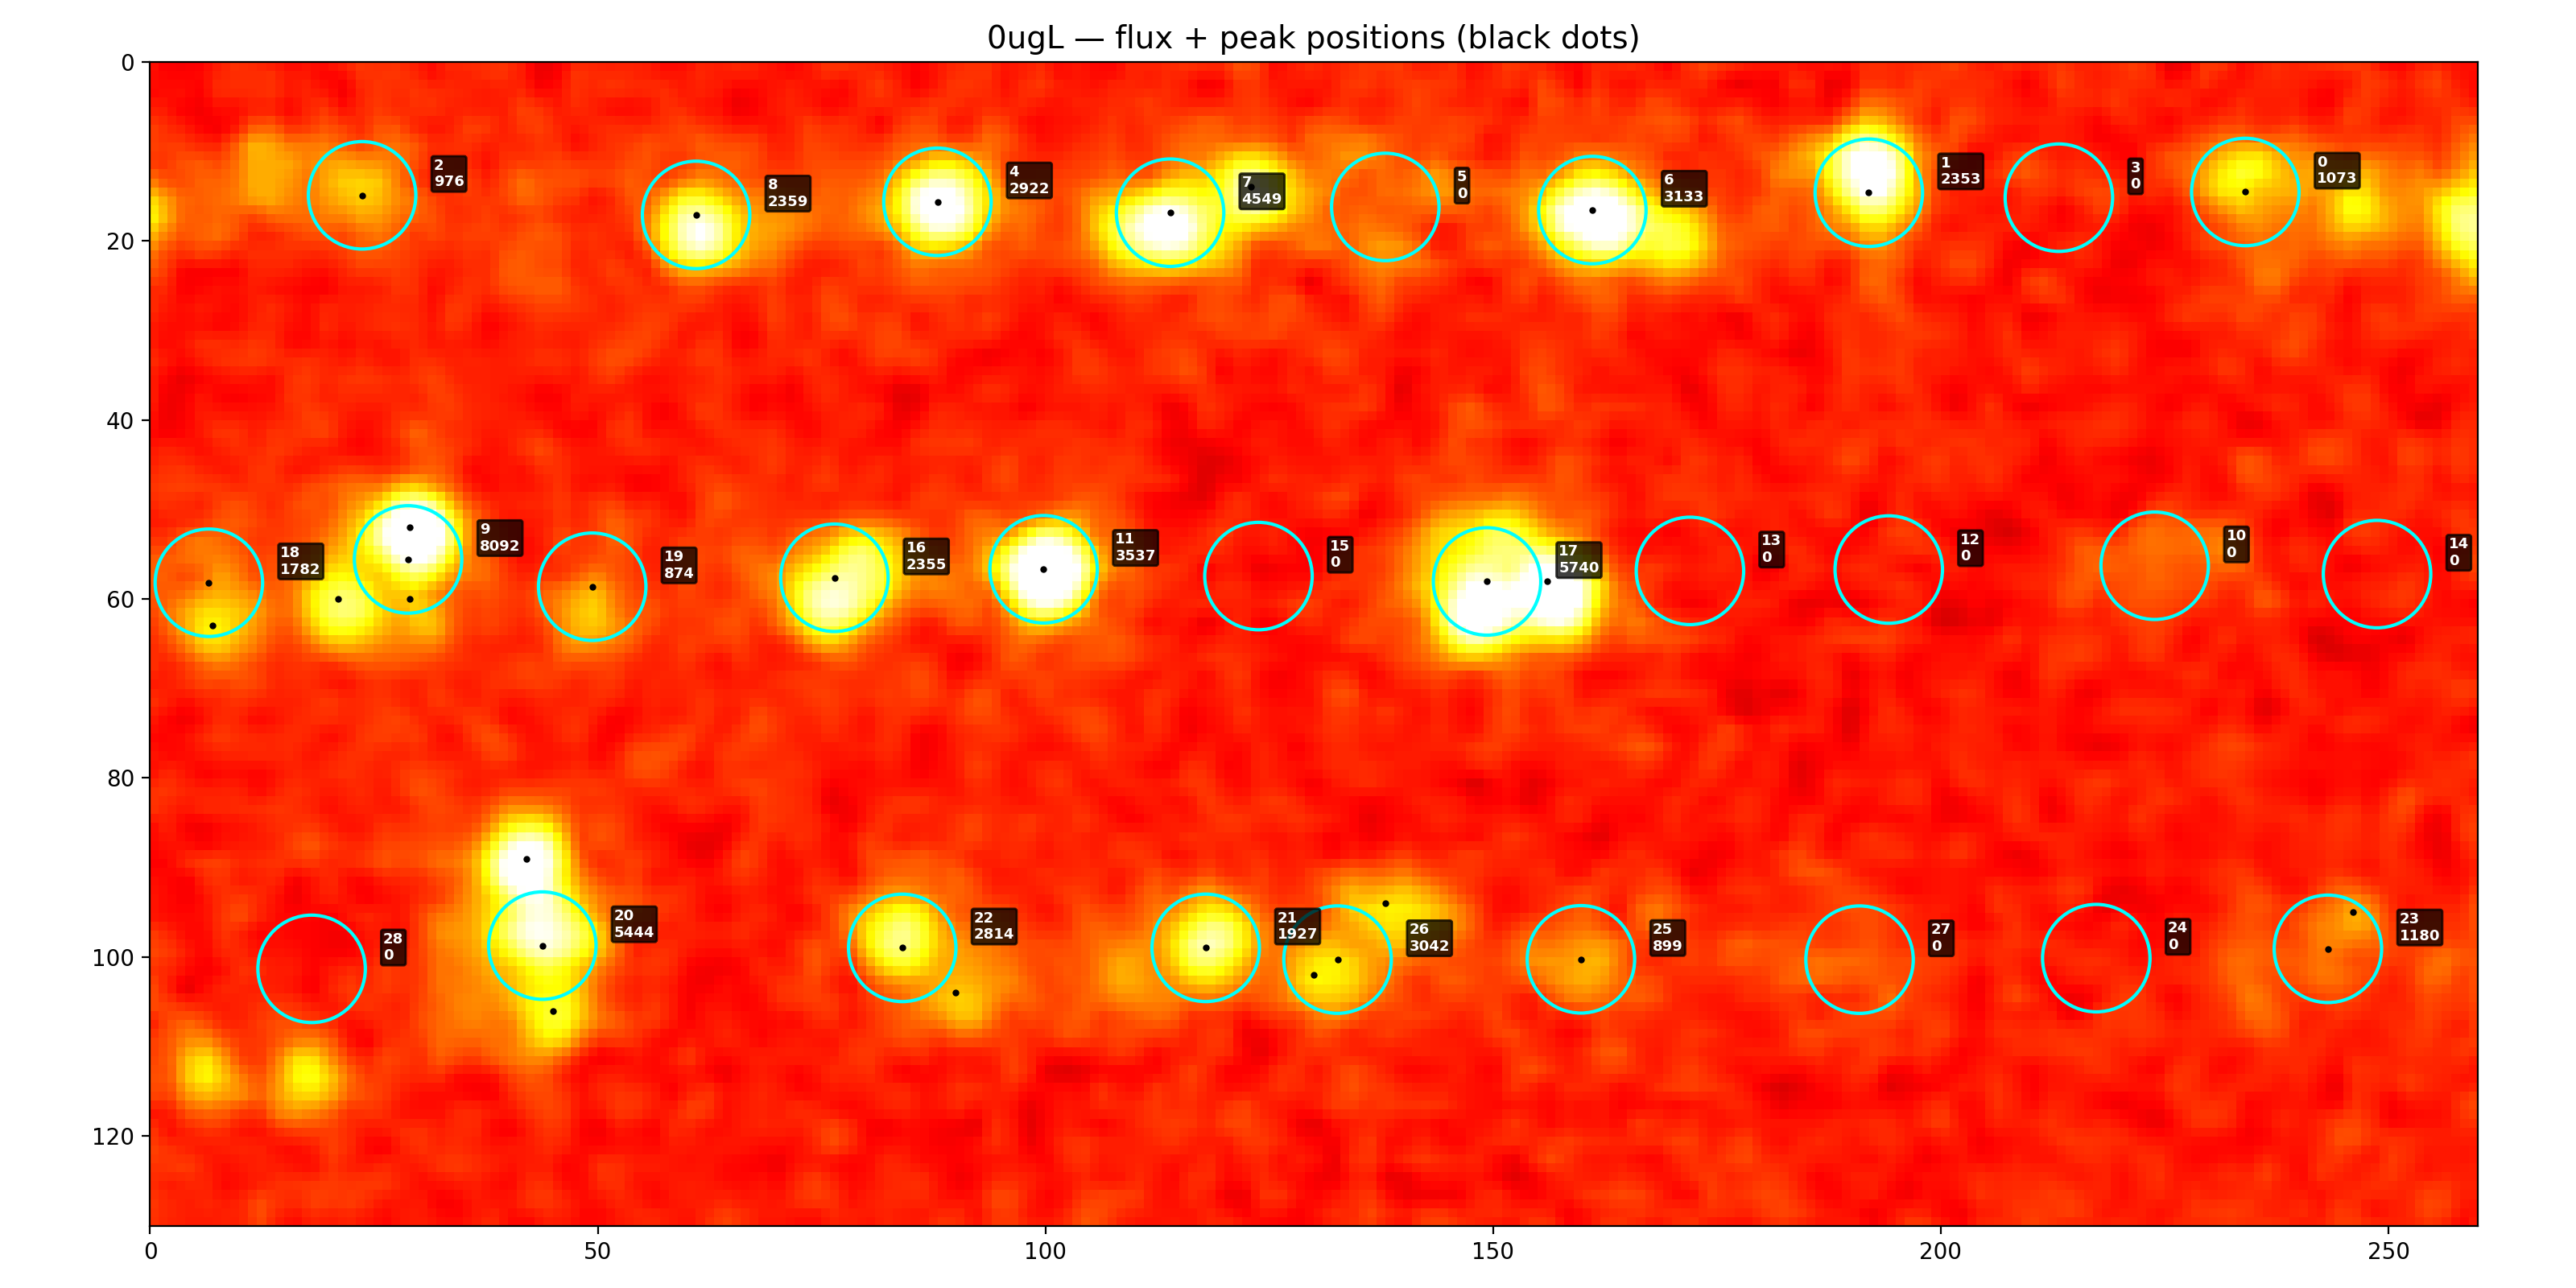
\includegraphics[width=\textwidth]{../figures/crop/_crop_numbered_0ugL.png}
    \caption{0\,$\mu$g/L}
\end{subfigure}
\hfill
\begin{subfigure}[b]{0.32\textwidth}
    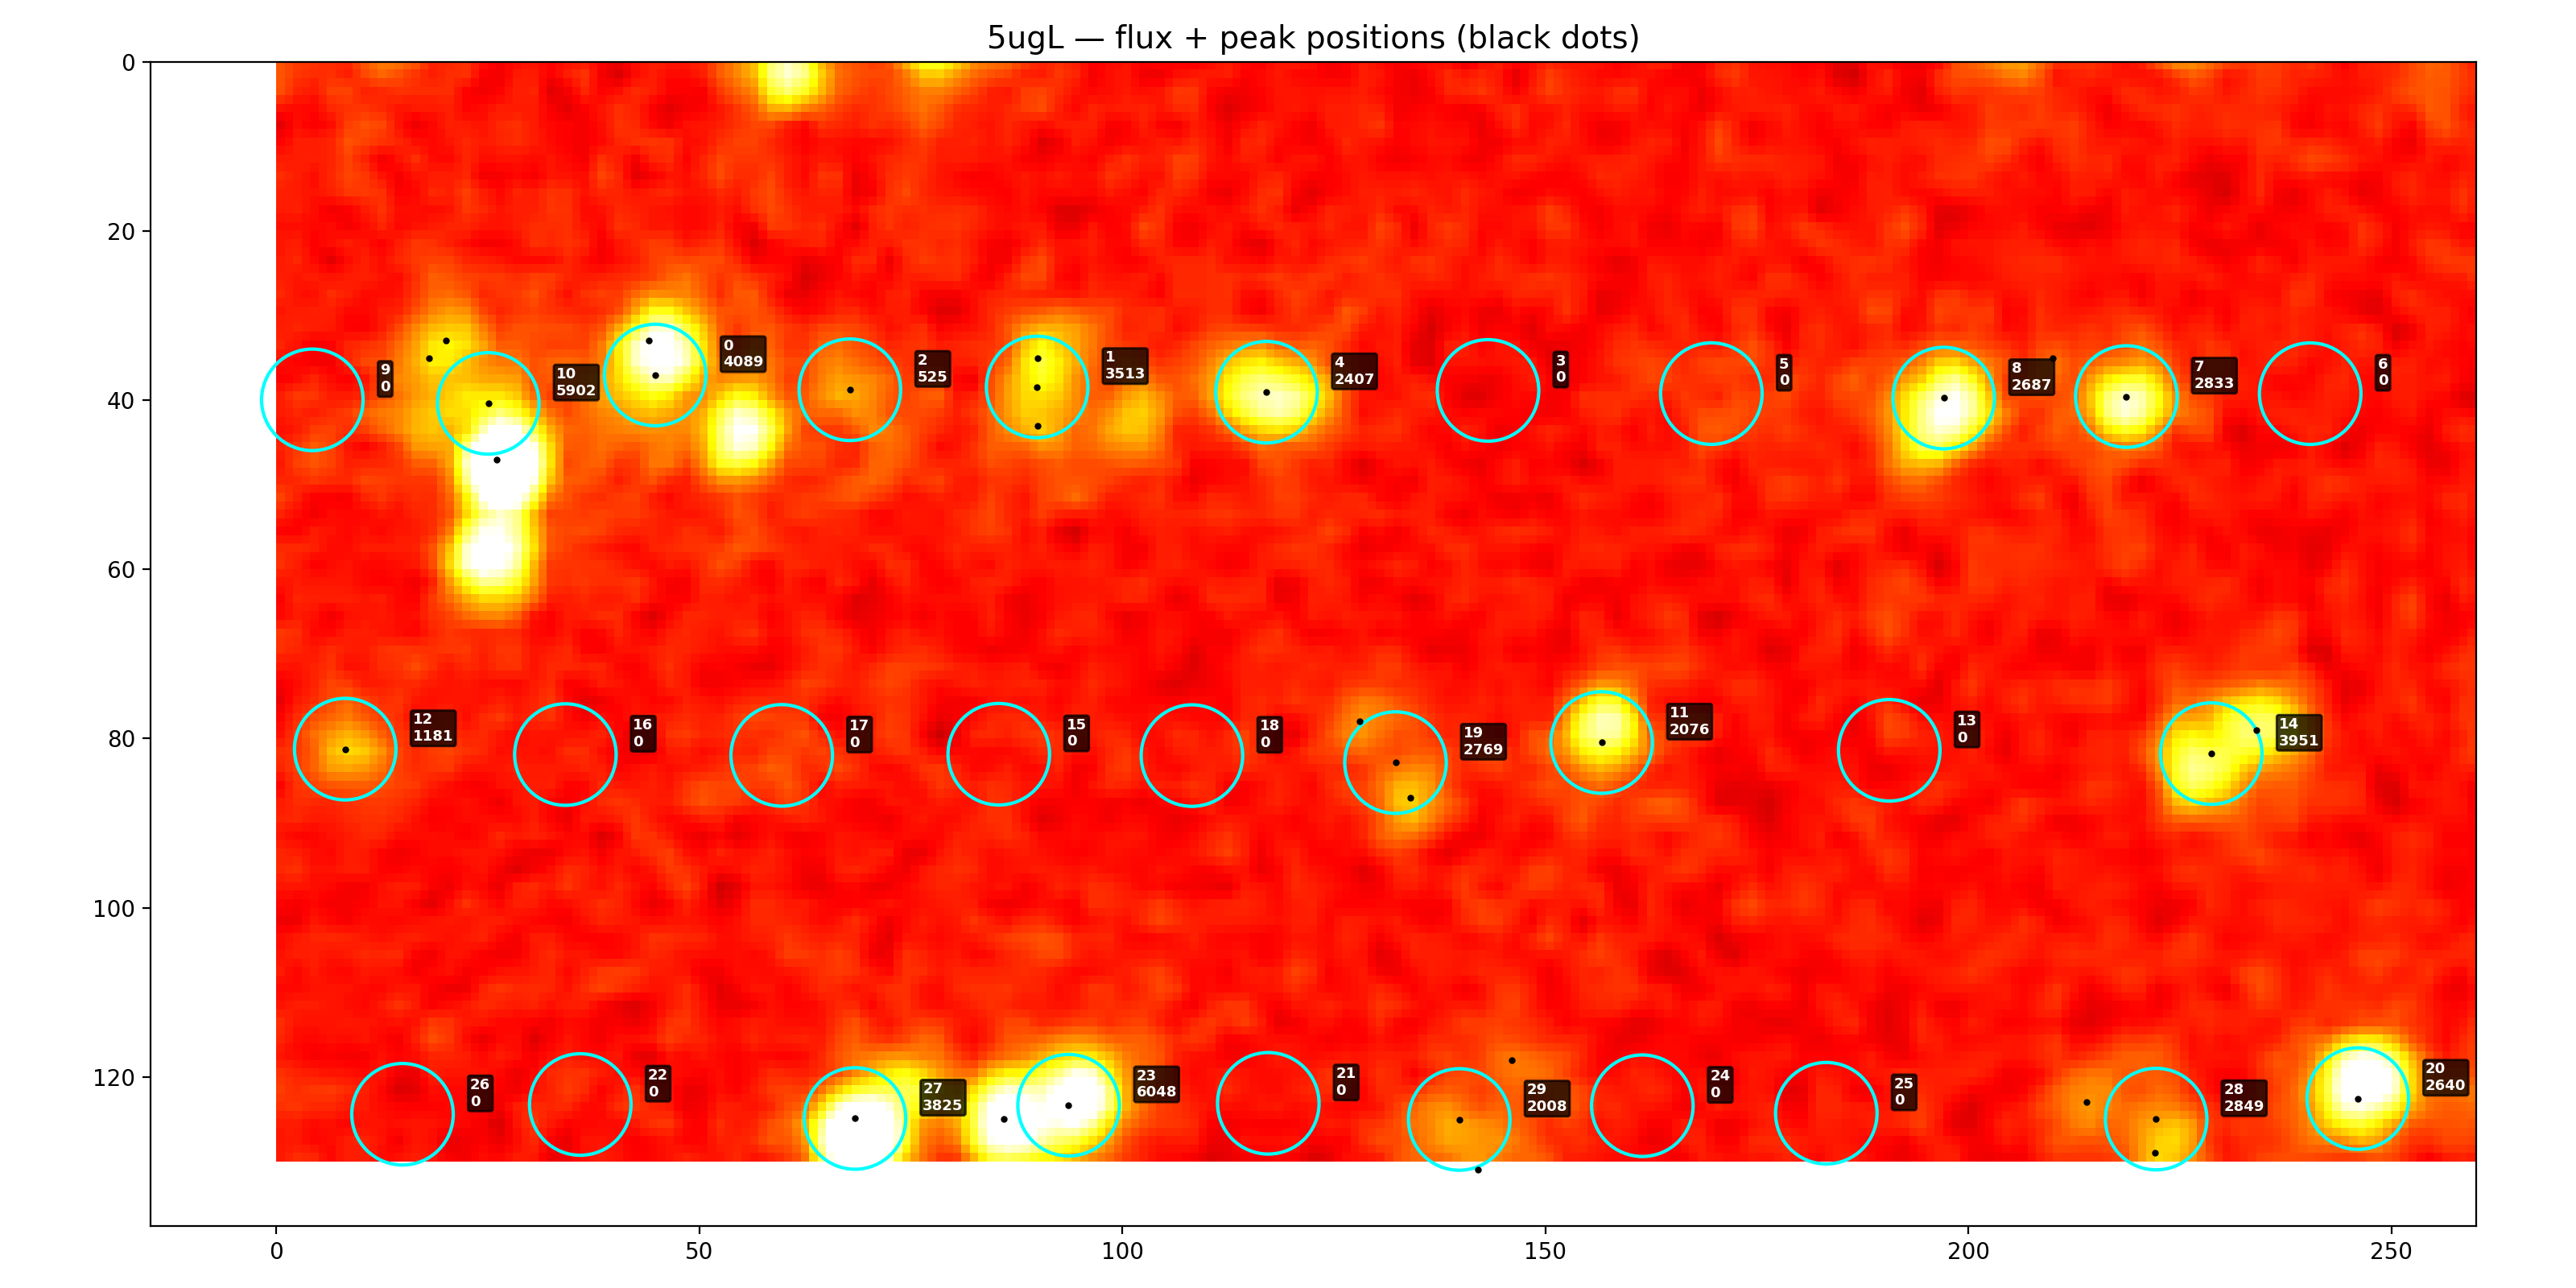
\includegraphics[width=\textwidth]{../figures/crop/_crop_numbered_5ugL.png}
    \caption{5\,$\mu$g/L}
\end{subfigure}
\hfill
\begin{subfigure}[b]{0.32\textwidth}
    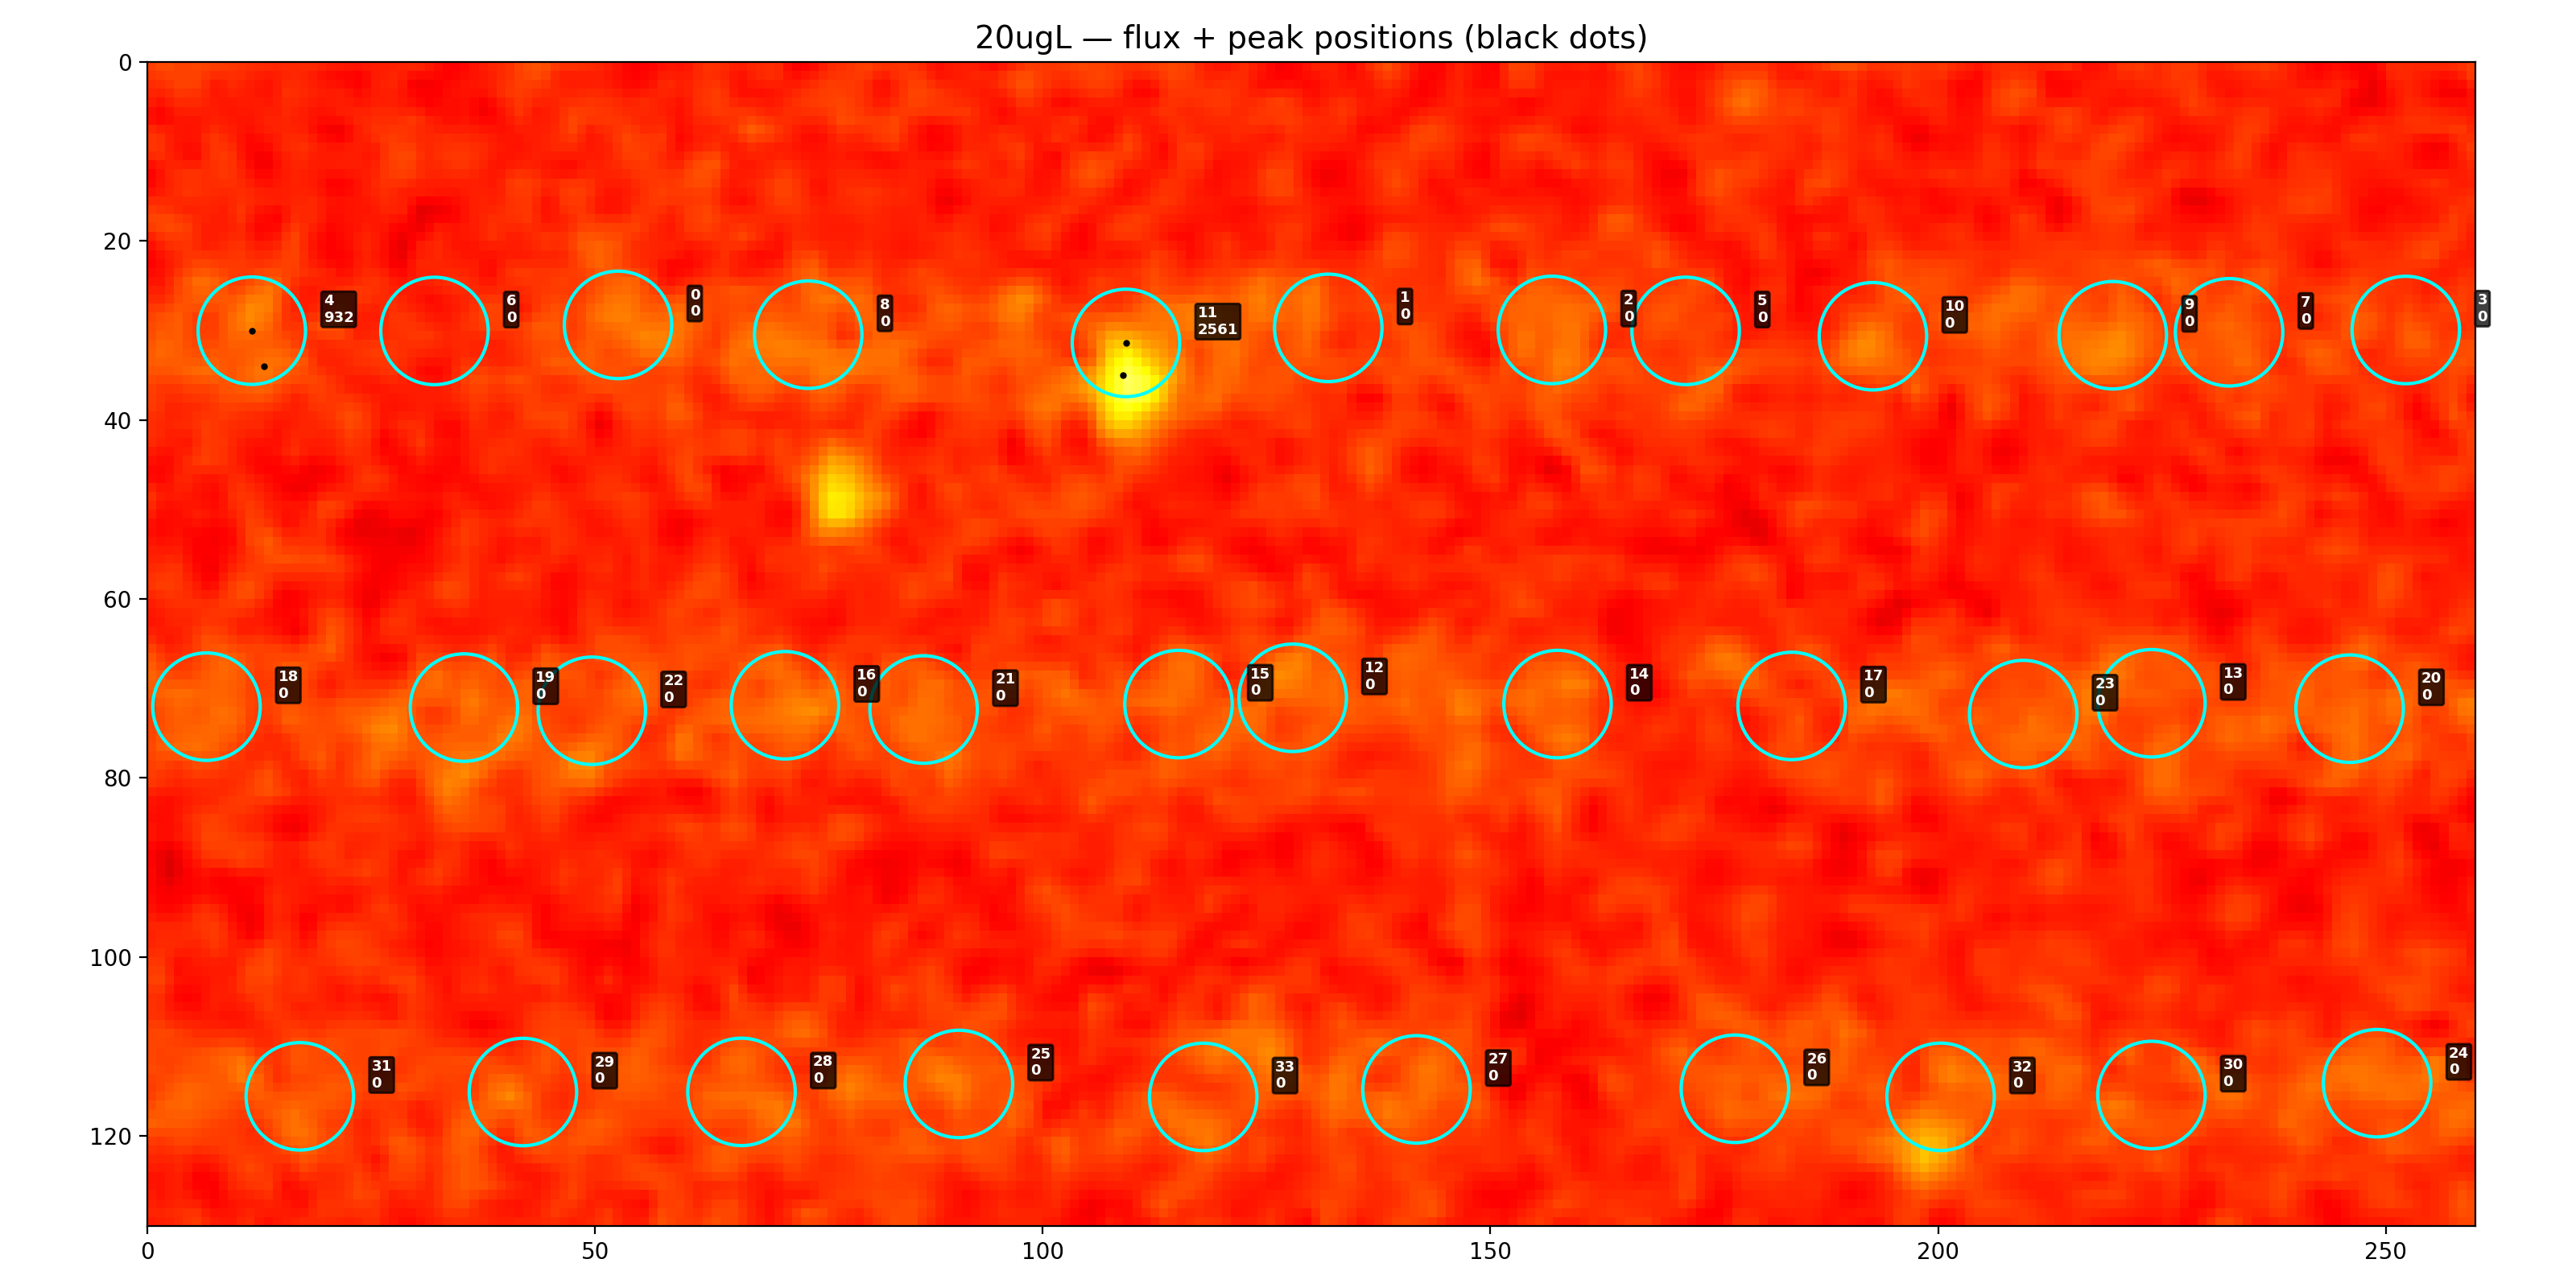
\includegraphics[width=\textwidth]{../figures/crop/_crop_numbered_20ugL.png}
    \caption{20\,$\mu$g/L}
\end{subfigure}
\caption{三种淬灭剂浓度下的荧光阵列局部检测结果。圆圈标注已定位的微孔位点及其通量值，黑点为峰值位置。随淬灭剂浓度升高，活性位点数量和亮度均显著下降。}
\label{fig:crop_detection}
\end{figure}

\begin{figure}[htbp]
\centering

\includegraphics[width=0.95\textwidth]{../figures/distribution/distributions_bar.png}
\caption{三种淬灭剂浓度下的五级离散荧光强度分布。0\,$\mu$g/L样品中淬灭位点占比约54.7\%，5\,$\mu$g/L升至77.5\%，20\,$\mu$g/L达到95.2\%，体现了荧光淬灭效应随浓度的单调增强。}
\label{fig:distributions}
\end{figure}

\begin{figure}[htbp]
\centering
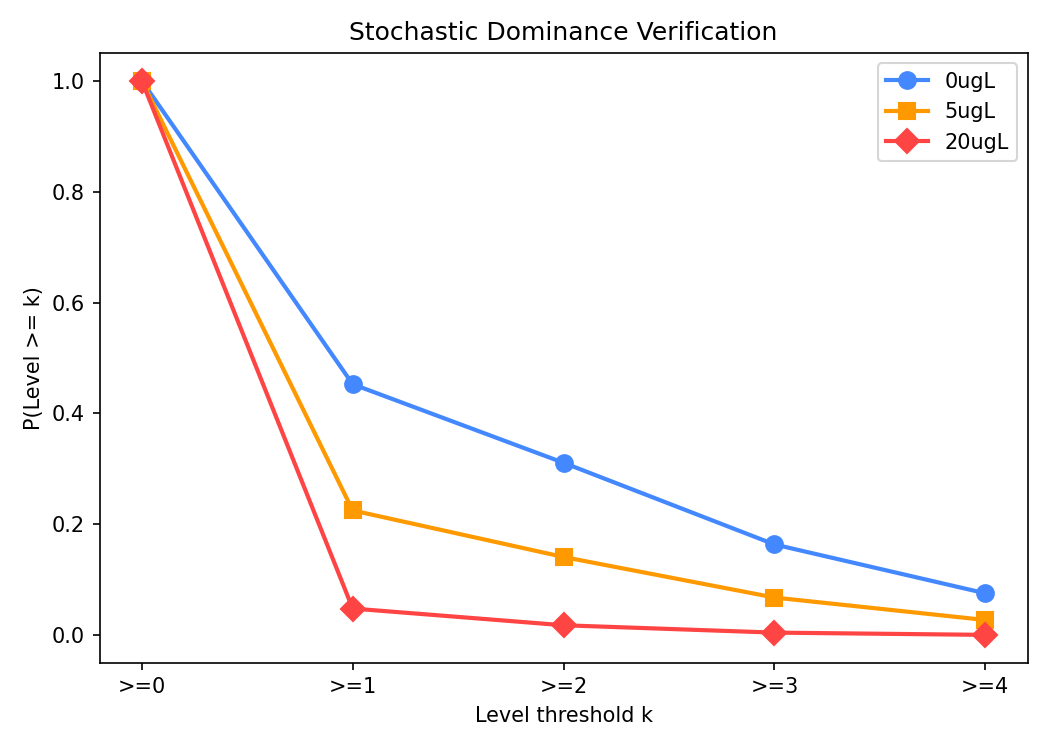
\includegraphics[width=0.55\textwidth]{../figures/distribution/stochastic_dominance.png}
\caption{随机占优检验结果。累积超越概率$P(\text{Level} \geq k)$在所有阈值$k$处均满足$P_{0} \geq P_{5} \geq P_{20}$的严格单调递减关系，验证了算法输出与淬灭物理机制的一致性。}
\label{fig:stochastic_dominance}
\end{figure}

\subsection{样机开发与系统集成}

算法和仿真的最终价值必须通过硬件载体来体现。在完成光学机理仿真和全部信号处理算法的开发验证后，课题组将技术成果向硬件端输出，依托凌力教授课题组博士研究生王金鑫搭建的超材料光纤制备与加工平台以及便携式检测样机，完成了从"算法可用"到"设备可用"的关键跨越。整体工作沿两条并行路径推进：一是在标准光学平台上搭建宽谱光纤拉曼原理概念机，完成核心光路的原理验证和参数标定；二是将算法与仿真模型嵌入王金鑫已自主研发的便携式检测样机，在不增加硬件成本的前提下实现检测性能的显著提升，形成可部署、可操作的完整检测系统。

\subsubsection{光学平台上的原理概念机}

基于宽谱光纤拉曼检测思路，本项目在标准光学平台上搭建了一套原理性概念样机，作为核心光路验证和参数标定的实验基础。系统由光纤耦合激光光源、准直与聚焦光学组件、光纤探头及样品池模块、后向散射收集单元和光纤连接的拉曼光谱仪构成，各元件通过可调支架和精密位移台实现光路的多维对准。激发光经准直后耦合入光纤探头，在水样中激发宽谱拉曼散射信号，散射光再由同一探头返回，经滤光与聚焦后送入光谱仪，实现可见--近红外波段的宽谱拉曼响应测量。该概念机已完成基本光路调试和功能验证，能够在实验室条件下稳定获取典型溶液的拉曼特征峰。更重要的是，课题组在该平台上系统验证了COMSOL仿真给出的最优镀层参数和光纤结构参数，确认了仿真预测与实验测量之间的定量一致性，为后续便携式光纤拉曼检测装置的小型化集成和性能优化提供了经过实验校核的原型依据。

\subsubsection{便携式光学检测样机}

在前述光学仿真、信号处理算法和原理概念机验证全部完成后，本课题将全部算法与仿真模型整合嵌入至王金鑫已自主研发的水体新污染物便携式光学检测设备，实现了从分散算法模块到完整检测系统的集成。该设备由王金鑫前期独立完成整体方案设计、光路搭建及硬件调试，已具备在水环境中开展痕量新污染物检测的基础性能，是本便携式光学检测样机的工程基础。

样机以拉曼与荧光检测为核心光学机理，由激光光源、物镜和CMOS光电传感器构成基本光学链路，并通过前端可更换耦合单元，与光纤探头、免疫芯片等不同形式的检测界面实现统一对接。得益于设备方案中对光路复用和结构模块化的设计思路，同一套硬件平台既能承载宽谱拉曼测量所需的光纤检测单元，也能完成微流控免疫芯片的荧光读出，从而实现光学路径、探测器和数据采集系统的全面复用——这一"一平台、双模式"的硬件架构正是本项目"筛查--确证"闭环检测方案的物理载体。

本研究开发的光学机理仿真与全套信号处理算法嵌入该设备后，带来了三方面可量化的性能提升：\textbf{（1）}ALSL拉曼背景扣除算法显著改善了复杂水样中弱拉曼峰的信噪比，使检测限实质性降低；\textbf{（2）}荧光阵列自动化读出算法实现了单张芯片超过12\,000个微孔位点的全自动定量分析，处理时间仅数十秒，子区域读出一致性CV低至0.022；\textbf{（3）}COMSOL仿真给出的最优镀层和量子点标记参数指导了光纤探头与免疫芯片的工艺优化，从硬件源头提升了光场与待测体系的耦合效率。上述算法赋能\textbf{在不增加任何硬件成本的前提下}，使该设备的综合检测性能实现了从"基础可用"到"高灵敏度、高通量、高一致性"的质的跃升，推动了这一便携式检测系统在流域现场监测和高频布点应用中具备真正的工程部署价值。需特别说明的是，本项目经费未用于设备硬件开发工作，该部分硬件平台归属王金鑫前期研究成果，本课题的贡献集中在算法嵌入与性能提升。

\section{项目目标完成情况}

总体来看，本课题\textbf{全面完成并在多个维度超越了}立项时设定的各项预期目标。

\textbf{在核心技术层面}，项目实现了从光学机理仿真、信号处理算法开发到便携式样机集成的全链条贯通：基于COMSOL建立了光纤倏逝波和量子点界面两类仿真模型并给出工程化设计准则；开发了ALSL拉曼背景扣除、转移矩阵荧光分布演化解析、多角度复折射率反演以及荧光阵列自动化读出等四套核心算法，构建了从原始信号到物性参数与机理解释的完整数据处理体系；在同一便携硬件平台上实现了宽谱拉曼与量子点荧光的双模式检测，设备综合成本仅为传统液相色谱--三重四极杆质谱系统的约百分之一，单次检测通量提升百倍以上。上述成果不仅全面达到了立项时设定的"形成可运行原型、证明技术路线可行"的基本目标，更从灵敏度、通量和自动化程度等方面实现了显著超越。

\textbf{在学术成果层面}，项目产出了具有国际影响力的高水平研究成果：核心算法已在\textit{Journal of Hazardous Materials}发表的合作论文中得到外部验证，另有论文投稿至\textit{Nature Communications}（已完成第一轮同行评审）和\textit{Nature Sustainability}（审稿中），形成1件发明专利，充分体现了项目在学术原创性和技术前沿性方面的竞争力。

\textbf{在产业化与商业化层面}，项目成果远超立项时"初步探索应用场景"的预期：已与安利（中国）、科德宝过滤技术集团、深圳中科先见医疗科技、广州谱临晟科技等四家行业头部企业达成产业化合作意向，形成了覆盖C端消费品、B端工业水处理、医疗器械和光学仪器制造的完整产业协同布局，完成了商业模式架构设计和商业计划书，并在代表性场景中开展了初步验证，为后续规模化推广奠定了坚实基础。

\section{项目成果与经验总结}

\subsection{项目实施中遇到的困难与解决经验}

项目实施过程中遇到的主要困难集中在以下几个方面，团队通过持续探索和迭代优化，将每一个技术瓶颈转化为推动方案升级的驱动力：

\subsubsection{从模拟水样到真实水体：复杂基质下的信噪比挑战}

项目初期，算法与样机主要在去离子水配制的标准溶液上完成了灵敏度与检测限的初步验证，结果符合预期。然而，当团队将检测对象切换至含有大量有机质、悬浮颗粒和多种共存离子的真实环境水样时，荧光本底急剧抬升，拉曼特征峰几乎被淹没，原有算法的检测性能出现断崖式下降。这一"实验室到现场"的鸿沟迫使团队从算法层面重新审视问题：正是在解决真实水样背景干扰的过程中，ALSL自适应背景扣除算法被开发并持续优化，最终实现了在复杂非线性背景下对弱拉曼峰的稳定提取。同样，荧光阵列读出算法也在真实样品的激发光场不均匀性和量子点多分支发射等问题的驱动下，经过多轮迭代升级，最终形成了包含几何校正、淬灭位点恢复和两阶段无重叠积分的成熟方案。这一经历使团队深刻认识到，算法的真正价值不在实验室的理想条件下，而在于面对真实场景复杂性时的鲁棒性。

\subsubsection{从"能用"到"好用"：便携化样机的工程化瓶颈}

宽谱光纤拉曼概念机在标准光学平台上运行稳定，但将其向便携化方向推进时，光路对准精度、环境温度波动对光谱基线的影响、以及长时间运行后光源功率漂移等工程化问题逐一暴露。团队依托COMSOL仿真给出的参数优化图谱，有针对性地调整了镀层结构和光纤耦合参数，并在信号采集端引入内置参考光源进行实时标定，在不牺牲检测灵敏度的前提下有效提升了系统的环境适应性和长时间运行稳定性。这一过程让团队积累了从实验室原型到工程化产品之间的宝贵经验：仿真优化的最终价值必须通过硬件验证来兑现，而工程化问题的解决往往反过来为仿真模型提供更精确的边界条件。

\subsubsection{从单一目标物到检测谱系：标准物质与方法数据库的构建}

单一目标物的检测验证相对容易实现，但构建覆盖多类新污染物的检测谱系则面临标准物质获取困难、不同目标物光谱响应差异大、基质效应复杂等系统性挑战。团队采取了"核心算法通用化+检测参数目标物特异化"的分层策略：将ALSL背景扣除、荧光阵列读出和转移矩阵解析等核心算法封装为与目标物无关的标准化工具，同时针对每类目标物建立专属的光谱响应库和定量校准曲线。围绕典型抗生素和模型污染物，团队逐步建立了涵盖多类目标物和典型基质条件的标准物质与实测样本数据库，为算法的跨场景迁移和检测谱系的持续扩展奠定了数据基础。

\subsubsection{从技术验证到产业落地：跨行业合作模式的探索}

技术研发与产业化落地之间存在巨大的认知鸿沟：实验室关注的是检测限和信噪比，而企业关注的是成本、产能、法规合规和用户体验。团队在与安利、科德宝、中科先见、谱临晟等企业的对接过程中，切身体会到不同行业对同一技术的需求差异——消费品企业关注的是终端用户的操作便捷性，工业过滤企业关注的是与现有产线的兼容性，医疗器械企业关注的是注册认证路径。这些来自产业端的反馈反向推动了团队对技术方案模块化、接口标准化和合规性设计的重视，也使团队在项目后期的商业模式设计中能够更加贴近真实市场需求。

\subsection{已取得的主要成果}

依托项目全周期的系统工作，本课题在技术研发、学术产出和产业化探索三个维度均形成了具有标志性意义的代表性成果：

\subsubsection{可复用的光学仿真模型库与工程设计准则}

基于COMSOL有限元仿真平台，建立了光纤倏逝波--镀层结构耦合模型和量子点标记界面局域光场模型两大核心仿真体系，形成了包含模型文件、参数扫描脚本和后处理工具在内的可复用仿真模型库。通过对纤芯/包层材料、镀层厚度与折射率、量子点负载密度等关键参数的系统扫描，明确了"高灵敏度--低损耗"和"有效信号--可控背景"的最优参数窗口，汇总形成了面向工程设计的光学参数优化图谱。该成果已直接指导便携式样机的硬件选型与工艺优化，并为投稿至\textit{Nature Communications}的合作论文提供了核心仿真数据支撑。

\subsubsection{全链条信号处理算法体系与标准化检测流程}

开发了ALSL拉曼背景扣除、转移矩阵荧光分布演化解析、多角度复折射率反演以及荧光阵列自动化定量读出等四套核心算法，构建了从原始信号采集到物性参数标定与机理解释的完整数据处理链。其中ALSL算法已在\textit{Journal of Hazardous Materials}发表的论文中得到外部验证，复折射率反演算法已在投稿至\textit{Nature Sustainability}的论文中得到独立应用。围绕便携式检测原型系统，建立了涵盖硬件启动、光路校正、自动调焦、信号采集及算法处理的标准化检测流程，通过内置参考光源快速标定和统一参数设定，有效减小了不同批次芯片和操作人员之间的差异，使非专业人员经短期培训即可独立操作。

\subsubsection{真实场景检测数据集与标准物质数据库}

通过与环保部门、水务单位及合作企业的联合测试，在流域断面、污水处理关键节点以及特殊执法场景中，获取了覆盖多种水体类型和多类新污染物的真实环境检测数据集，并与传统色谱--质谱方法的检测结果进行了系统比对验证。在此基础上，建立了涵盖典型抗生素、模型污染物及多种基质条件的标准物质与实测样本数据库，配合已封装的标准化算法工具库，形成了可直接支持检测谱系扩展和算法跨场景迁移的数据基础设施。

\subsubsection{高水平学术论文与知识产权}

围绕便携式光学原位检测体系的光场调控机理、信号处理算法和超材料光纤结构优化等方向，项目产出了具有国际影响力的学术成果：\textbf{1篇论文已在环境科学领域权威期刊\textit{Journal of Hazardous Materials}正式发表}（项目负责人马泽炫为第四作者）；1篇论文投稿至\textit{Nature Communications}并已完成第一轮同行评审（马泽炫为第二作者）；1篇论文投稿至\textit{Nature Sustainability}（马泽炫为第八作者）。在知识产权方面，已形成1件发明专利，并在现有成果基础上进一步凝练了具有推广潜力的新专利点和算法相关软件著作权，为后续成果转化夯实了知识产权基础。

\subsubsection{产业协同布局与创业雏形}

在模拟创业与企业雏形建设方面，已构建了以"水环境新污染物便携式检测解决方案提供商"为核心的完整商业体系：形成了"设备切入--耗材锁定--数据增值"三级递进商业模式、较为完整的商业计划书和路演材料，并与安利（中国）、科德宝过滤技术集团、深圳中科先见医疗科技、广州谱临晟科技等四家横跨消费品、工业过滤、医疗器械和光学制造领域的行业头部企业达成产业化合作意向，初步实现了从核心技术研发到产业化路径构建再到多市场落地模式设计的完整闭环。通过项目全过程训练，培养了一批兼具环境科学、光学工程与创新创业素养的复合型本科生，为学校在新污染物治理与高端装备领域的人才储备和学科交叉发展提供了有力支撑。

\section{对学生创新思维和综合能力培养的作用}

本项目以"面向水体新污染物的高性能便携式光学检测方案"为主线，完整覆盖了从基础科学问题提出、关键技术攻关、原型系统搭建到商业模式设计的全链条，要求学生在同一个项目周期内同时扮演研究者、工程师和创业者三重角色。这种高强度、多维度的实践训练，对学生创新思维和综合能力的培养产生了深刻而全面的影响。

\subsection{强化问题导向的创新意识}

学生不是从"技术本身"出发，而是从国家新污染物治理的战略需求和现有检测体系"高灵敏度与高便携性难以兼顾"的结构性矛盾出发，思考如何用光学检测+算法优化的技术路径打破这一僵局。例如，荧光阵列自动化读出算法的开发，正是源于团队在实际测试中发现单张芯片12\,000余个微孔位点无法通过人工判读完成定量分析这一现实瓶颈，而非单纯的算法兴趣。在此过程中，学生逐步形成了"先看场景和需求、再选技术路径和实现形式"的工程创新思维，学会用系统视角审视技术方案的价值，而不是停留在单一指标的追求上。

\subsection{提升跨学科综合运用能力}

本项目天然地要求学生跨越多个学科边界：COMSOL光场仿真涉及电磁学与数值计算方法，ALSL算法涉及信号处理与最优化理论，转移矩阵解析涉及概率论与反问题求解，免疫芯片制备涉及材料化学与生物功能化，而整个检测方案的应用场景则根植于环境科学对新污染物赋存与迁移行为的认识。学生在项目中被迫走出自己的专业舒适区——物理学背景的成员需要理解免疫识别的生物化学原理，计算机背景的成员需要理解光学信号的物理来源。这种真实驱动的跨学科融合，远比课堂教学中的跨学科概念更加深入和持久。

\subsection{锻炼工程实践与系统集成能力}

围绕便携式光学检测系统的构建，学生亲历了从仿真预测到实验验证、从实验室概念机到便携式样机的完整工程化过程。在这一过程中，学生切身体会到实验室中"能工作"与工程上"可部署"之间的巨大鸿沟——仿真给出的最优参数在实际光路中可能因加工公差而偏移，算法在理想数据上表现优异但在真实图像中面临光场不均匀和多分支PSF交叠等未预见的挑战。正是通过反复调试、验证和修正，学生形成了"设计--实验--反馈--迭代"的工程思维闭环，学会在性能、成本、体积和稳定性之间做出务实的工程权衡。

\subsection{增强科研素养与数据驱动思维}

项目全过程严格贯彻了科研规范：从文献检索与综述、实验对照组设计、空白校准与标准曲线建立，到误差传播分析和统计检验。尤其值得一提的是，荧光阵列读出算法的验证中，团队自主设计了子区域均匀性分析（CV指标）和随机占优检验两套独立的统计检验框架，这种"用严格的统计方法验证自己算法"的自我审视能力，已超越了一般本科生项目的科研深度。在处理三种浓度梯度、每张芯片超过12\,000个位点的海量数据过程中，学生深刻体会到数据驱动决策的力量——不是靠主观感觉判断算法好坏，而是让统计检验给出客观回答。

\subsection{培养创新创业意识和面向社会的责任感}

在项目后半段，团队从纯技术研发角色切换至"解决方案设计者"角色，围绕水环境监测、食品安全、公共健康和执法缉毒等不同应用场景，构思了从B端政府采购到C端家庭快检的多层次产品形态，并与安利、科德宝等行业头部企业进行了真实的商务技术对接。这一经历让学生深刻认识到：技术的价值不止于论文和专利，更在于能否转化为解决真实社会问题的产品和服务。同时，围绕新污染物治理、水环境安全和公共健康等议题的深入接触，使学生建立起强烈的环保意识和社会责任感——他们所做的工作，直接关系到数以亿计民众的饮用水安全。

\subsection{提升团队协作、沟通与项目管理能力}

项目实施过程中，5名本科生成员需要在光学仿真、算法开发、实验验证、报告撰写和外部企业对接等多条战线上同步推进，并与指导教师凌力教授和博士生王金鑫保持密切协同。学生在分工协作中逐步建立了清晰的里程碑意识和任务分解能力——每个成员不仅需要完成自己的技术模块，还需要理解上下游模块的接口和约束，才能确保整个系统的顺利集成。在多次项目汇报、路演展示和企业对接中，学生的书面表达、口头汇报和跨专业沟通能力得到了系统性锻炼，为其未来进入科研或产业领域奠定了扎实的综合素养基础。

% ===== 参考文献 =====
\newpage
\begin{thebibliography}{20}

\bibitem{ref1} 国务院办公厅. 新污染物治理行动方案[EB/OL]. 北京：国务院，2022.

\bibitem{ref2} 中共中央，国务院. 关于全面推进美丽中国建设的意见[EB/OL]. 2023.

\bibitem{ref3} 科技部等. "十四五"生态环境领域科技创新专项规划[EB/OL]. 2022.

\bibitem{ref4} Browne A J, Chipeta M G, Haines-Woodhouse G, et al. Global antibiotic consumption and usage in humans, 2000--18: a spatial modelling study[J]. \textit{Lancet Planetary Health}, 2021, 5(12): e893--e904.

\bibitem{ref5} Guo Y, Liu S, Wang Z, et al. Radical chemistry and structural relationships of PPCP degradation by UV/chlorine treatment in simulated drinking water[J]. \textit{Environmental Science \& Technology}, 2017, 51: 10431--10439.

\bibitem{ref6} Han J, Zhang X, Liu J, et al. How much of the total organic halogen and developmental toxicity of chlorinated drinking water might be attributed to aromatic halogenated DBPs?[J] \textit{Environmental Science \& Technology}, 2021, 55(9): 5906--5916.

\bibitem{ref7} Klein E Y, Milkowska-Shibata M, Tseng K K, et al. Assessment of WHO antibiotic consumption and access targets in 76 countries, 2000--15: An analysis of pharmaceutical sales data[J]. \textit{Lancet Infectious Diseases}, 2021, 21(1): 107--115.

\bibitem{ref8} Minakata D, von Gunten U. Predicting Transformation Products during Aqueous Oxidation Processes: Current State and Outlook[J]. \textit{Environmental Science \& Technology}, 2023, 57(47): 18410--18419.

\bibitem{ref9} Murray C J L, Antimicrobial Resistance Collaborators. Global burden of bacterial antimicrobial resistance in 2019: A systematic analysis[J]. \textit{The Lancet}, 2022, 399: 629--655.

\bibitem{ref10} National Research Council (US) Committee on Research Opportunities in Biology. Opportunities in Biology[M]. Washington (DC): National Academies Press (US), 1989.

\bibitem{ref11} Ong T T X, Blanch E W, Jones O A H. Surface Enhanced Raman Spectroscopy in environmental analysis, monitoring and assessment[J]. \textit{Science of the Total Environment}, 2020, 720: 137601.

\bibitem{ref12} World Health Organization. Political Declaration of the High-level Meeting on Antimicrobial Resistance[R]. 2024.

\bibitem{ref13} Yue L, Zhao Y, Wang X, et al. Machine Learning-Assisted Molecular Structure Embedding for Accurate Prediction of Emerging Contaminant Removal by Ozonation Oxidation[J]. \textit{Environmental Science \& Technology}, 2025, 59(18): 9298--9311.

\bibitem{ref14} Eilers P H C, Boelens H F M. Baseline correction with asymmetric least squares smoothing[R]. Leiden: Leiden University Medical Centre, 2005.

\bibitem{ref15} Long D A. The Raman Effect: A Unified Treatment of the Theory of Raman Scattering by Molecules[M]. Chichester: John Wiley \& Sons, 2002.

\bibitem{ref16} Lakowicz J R. Principles of Fluorescence Spectroscopy[M]. 3rd ed. New York: Springer, 2006.

\bibitem{ref17} Yang Y, Wang J, Li L, et al. Unleashing the power of receptor-based assay on high-throughput detection: Assessing the feasibility of enzyme-linked immunosorbent assay on large-scale antibiotic monitoring[J]. \textit{Emerging Contaminants}, 2025, 11(3): 100511.

\end{thebibliography}

\end{document}
